\documentclass[11pt]{beamer}
\usetheme{CambridgeUS}

%-----------------------------------------------------------------------
% Packages
\usepackage[utf8]{inputenc}
\usepackage{amsmath}
\usepackage{amsfonts}
\usepackage{amssymb}
\usepackage{graphicx}
\usepackage{csquotes}
\usepackage{listings}
\usepackage{xcolor}
\usepackage{forest}

%-----------------------------------------------------------------------
% Package customization
\definecolor{links}{HTML}{FC0D30}
\hypersetup{colorlinks,linkcolor=,urlcolor=links}

\definecolor{coderegular}{rgb}{0.16, 0.16, 0.16}
\definecolor{codecomment}{rgb}{0.50, 0.35, 0.02}
\definecolor{codekeyword}{rgb}{0.5, 0.03, 0.09}
\definecolor{codestring}{rgb}{0.94, 0.34, 0.0}
\definecolor{codebackground}{rgb}{0.95,0.95,0.92}
\definecolor{codenumbers}{rgb}{0.5,0.5,0.5}

\lstdefinestyle{mystyle}{
    backgroundcolor=\color{codebackground},
    commentstyle=\color{codecomment},
    keywordstyle=\color{codekeyword},
    numberstyle=\tiny\color{codenumbers},
    stringstyle=\color{codestring},
    basicstyle=\ttfamily\footnotesize,
    breakatwhitespace=false,
    breaklines=true,
    captionpos=b,
    keepspaces=true,
    numbers=left,
    numbersep=2pt,
    showspaces=false,
    showstringspaces=false,
    showtabs=false,
    tabsize=2
}

\lstset{style=mystyle}

%-----------------------------------------------------------------------
% Commands
\renewcommand{\emph}[1]{\textbf{#1}}

%-----------------------------------------------------------------------
% Headings
\author{Marco Zanella}
\title{Introduction to Qt}
\setbeamercovered{transparent} 
\setbeamertemplate{navigation symbols}{} 
\logo{
\includegraphics[width=.05\textwidth]{assets/logo-unipd}} 
\institute{University of Padova} 
\date{December, 9, 2024} 
\subject{Course Structure} 

%-----------------------------------------------------------------------
% Document
\begin{document}

\begin{frame}
 \titlepage
\end{frame}

\begin{frame}
 \tableofcontents
\end{frame}


%-----------------------------------------------------------------------
\section{Overview}
\begin{frame}{Overview}
 What is Qt?
 \begin{displayquote}
  Qt (pronounced "cute") is cross-platform software for creating graphical user interfaces as well as cross-platform applications
  \begin{flushright}
  | \href{https://en.wikipedia.org/wiki/Qt_(software)}{Wikipedia}
  \end{flushright}
 \end{displayquote}
 
 \begin{figure}
  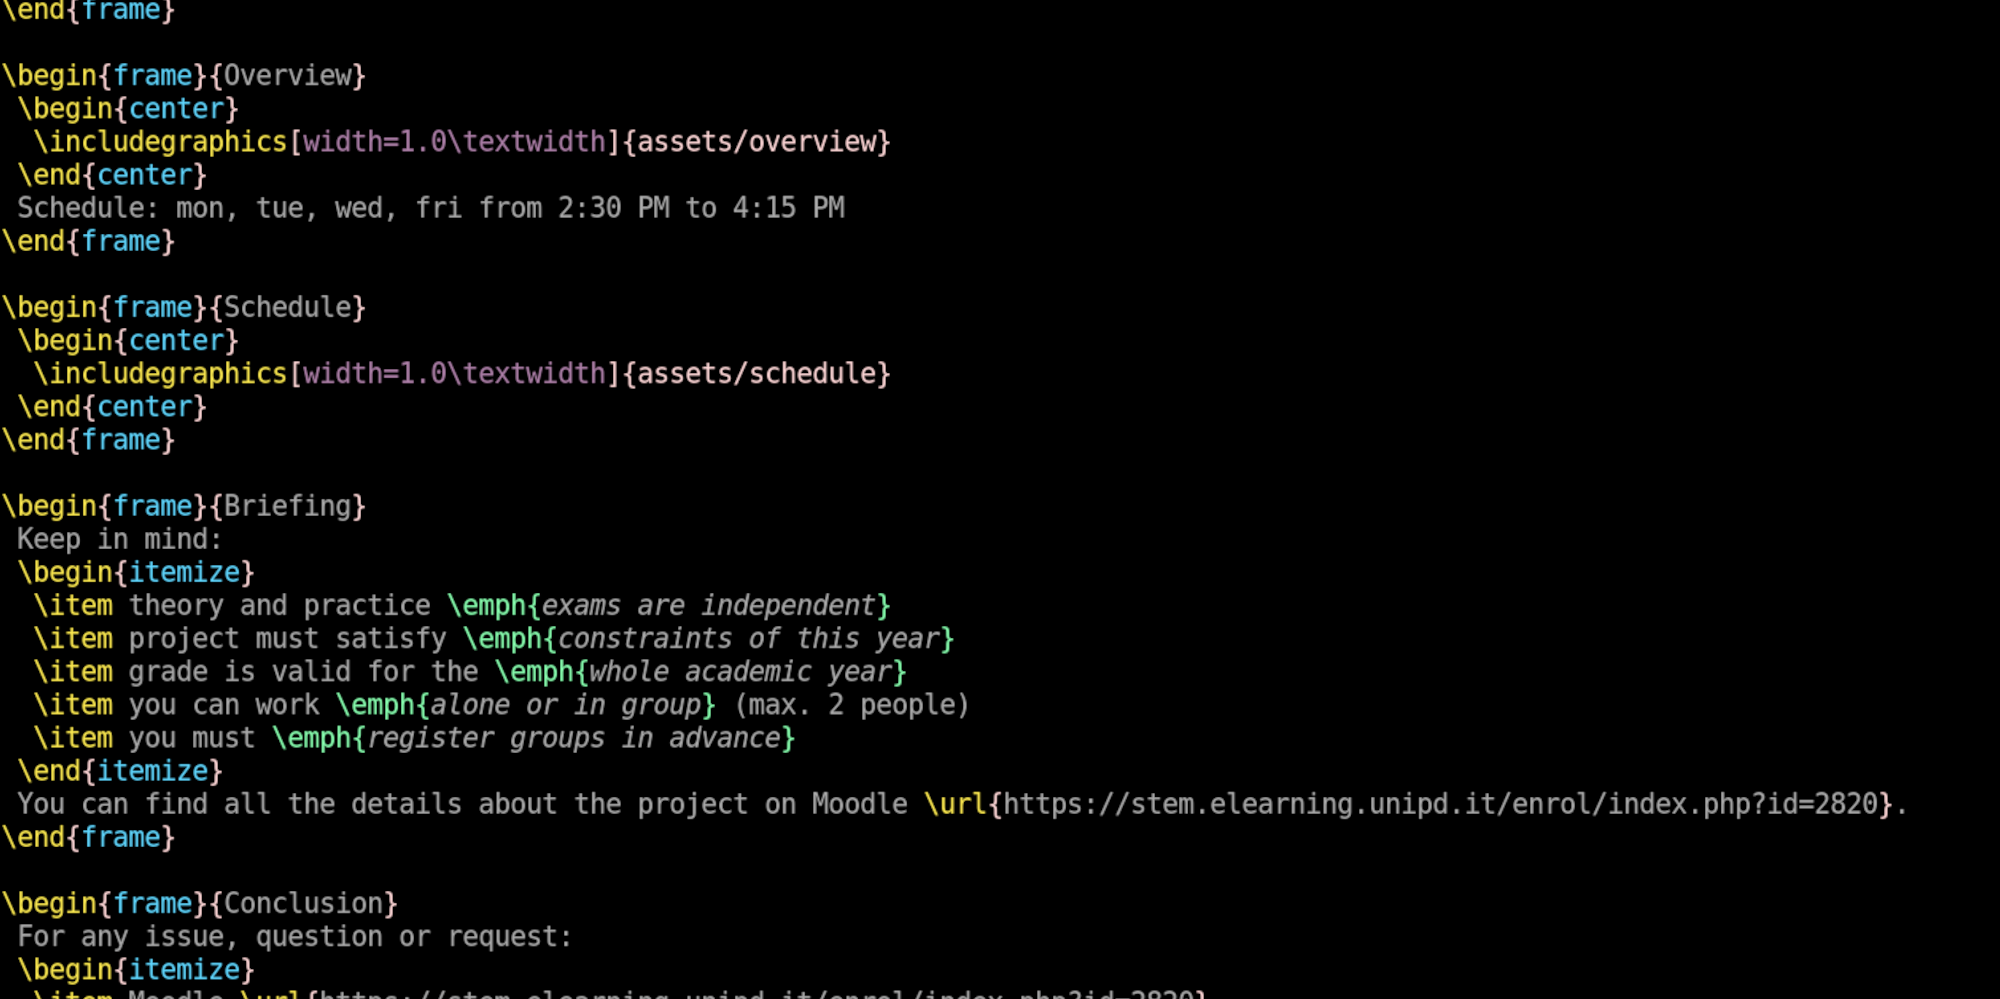
\includegraphics[width=0.45\textwidth]{assets/figure-cli}
  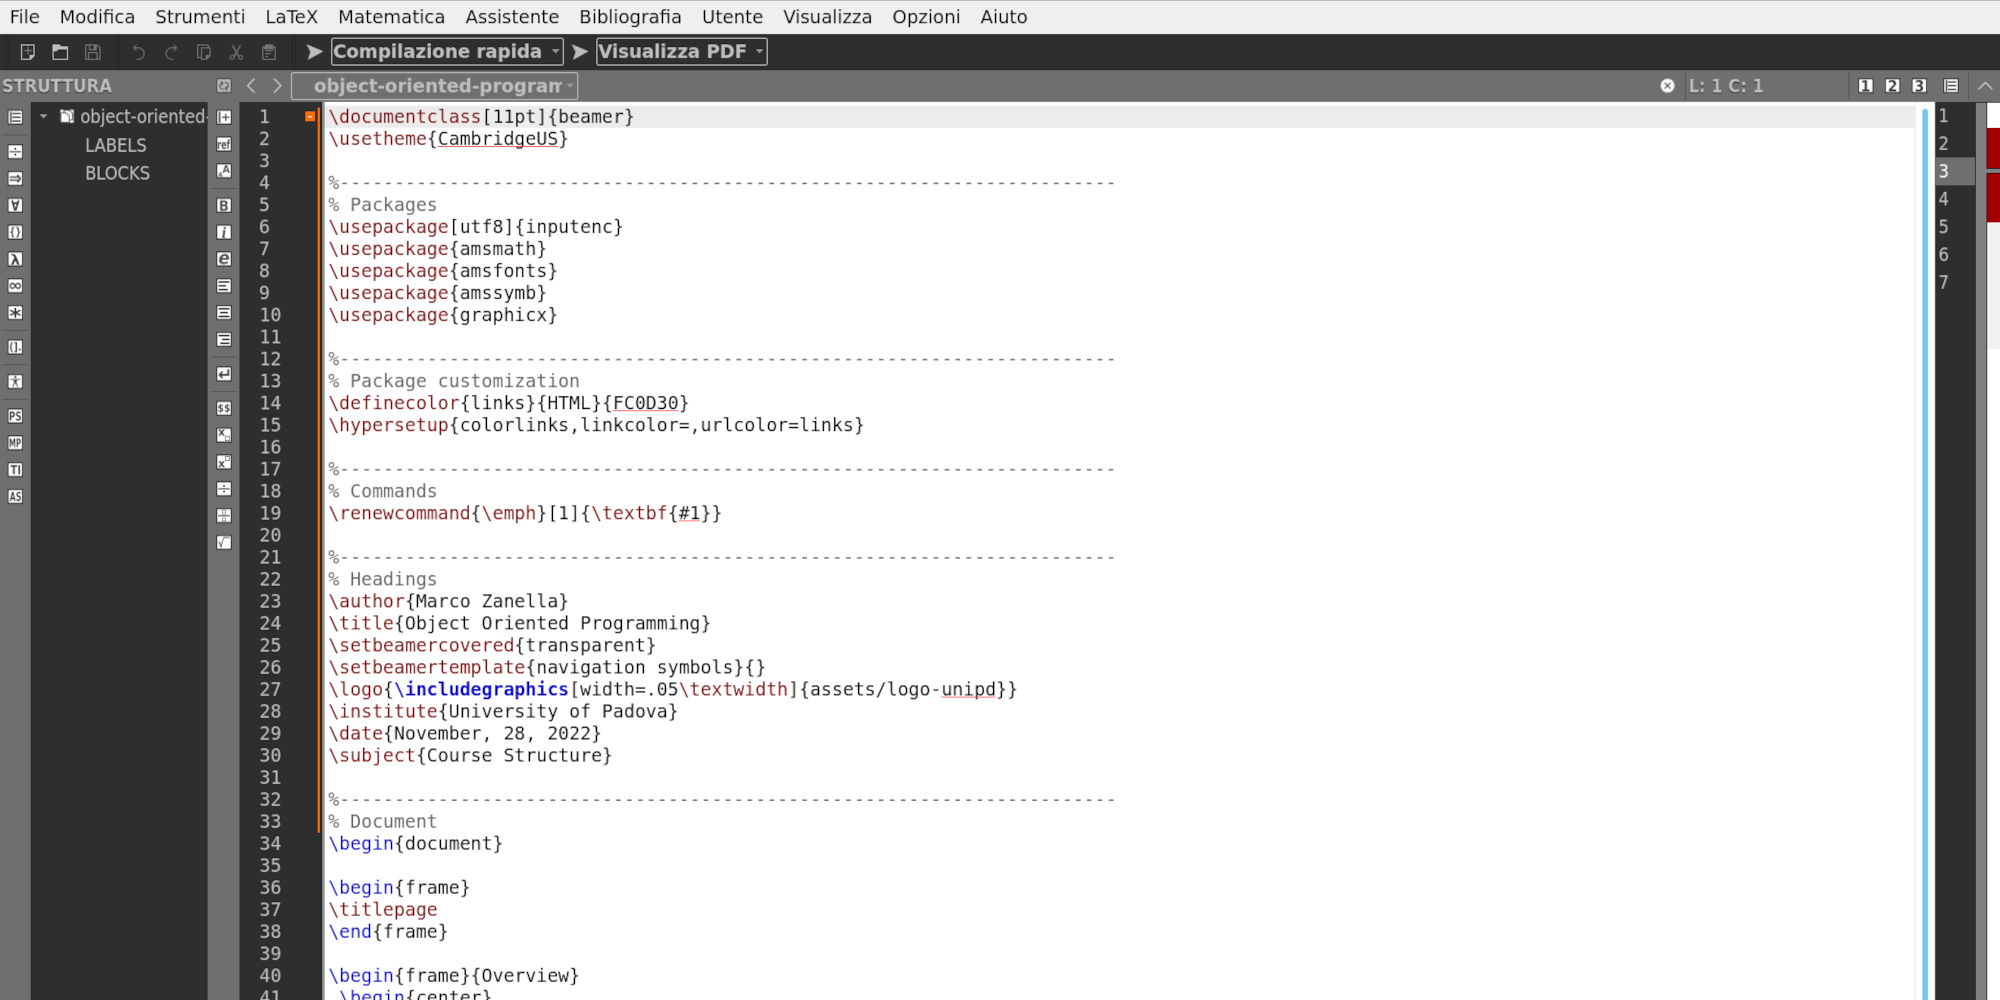
\includegraphics[width=0.45\textwidth]{assets/figure-gui}
 \end{figure}
 Qt allows to move from \emph{Command Line Interface} (CLI) to \emph{Graphical User Interface} (GUI).
\end{frame}

\begin{frame}{Overview / Motivation}
 Alternatives to Qt:
 \begin{figure}
  
\includegraphics[height=0.15\textheight]{assets/logo-gtk}
  
\includegraphics[height=0.15\textheight]{assets/logo-electron}
  
\includegraphics[height=0.15\textheight]{assets/logo-opengl}
  
\includegraphics[height=0.15\textheight]{assets/logo-vulkan}
 \end{figure}
 
 Why Qt?
 \begin{itemize}
  \item fully object oriented
  \item written in C++
  \item used by serious projects
 \end{itemize}
 
 Who uses Qt?
 \begin{figure}
  
\includegraphics[height=0.07\textheight]{assets/logo-3dstudiomax}
  
\includegraphics[height=0.07\textheight]{assets/logo-davinci-resolve}
  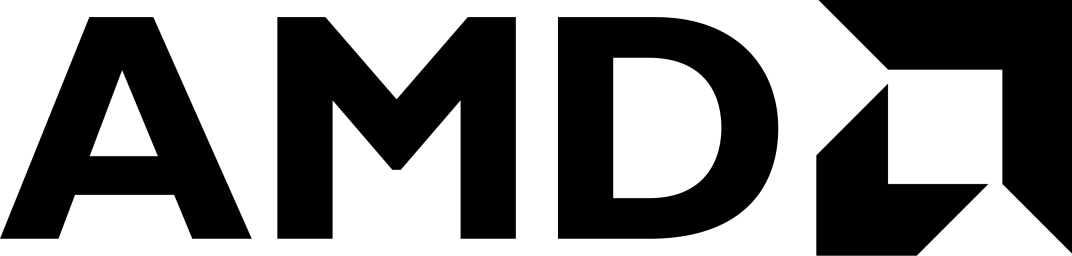
\includegraphics[height=0.07\textheight]{assets/logo-amd}
  
\includegraphics[height=0.07\textheight]{assets/logo-blizzard}
  
\includegraphics[height=0.07\textheight]{assets/logo-electronic-arts}
  
\includegraphics[height=0.07\textheight]{assets/logo-microsoft}
  
\includegraphics[height=0.07\textheight]{assets/logo-tesla}
  
\includegraphics[height=0.07\textheight]{assets/logo-walt-disney-animation-studios}
  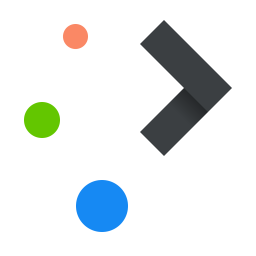
\includegraphics[height=0.07\textheight]{assets/logo-kde}
  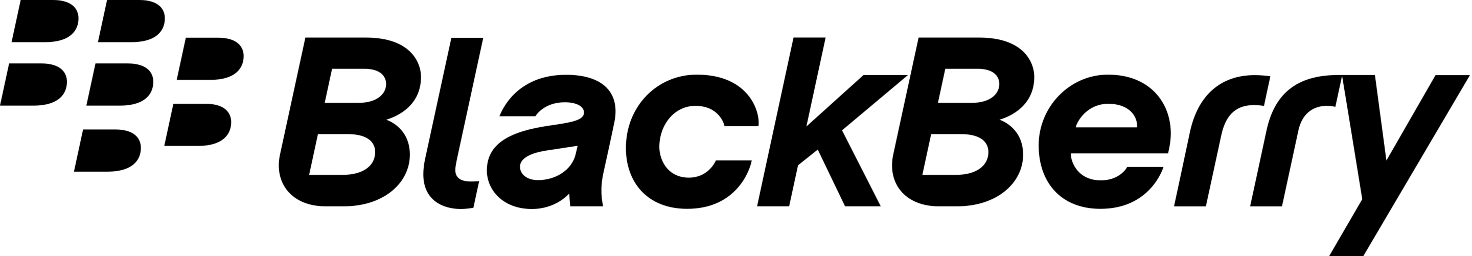
\includegraphics[height=0.07\textheight]{assets/logo-blackberry}
 \end{figure}
\end{frame}

\begin{frame}{Overview / Benefits}
 Additional benefits:
 \begin{itemize}
  \item containers
  \item SQL access
  \item XML and JSON support
  \item concurrent programming
  \item network programming
 \end{itemize}
\end{frame}

\begin{frame}{Overview / Primer}
 To get your application running:
 \begin{enumerate}
  \item install Qt
  \item write your code
  \item generate project file
  \item fix project file
  \item generate Makefile
  \item compile
  \item modify your code
  \item repeat from 5 or 6
 \end{enumerate}
 Check installation instructions for different OSs at \url{https://doc.qt.io/qt-5/gettingstarted.html}.
\end{frame}

\begin{frame}{Overview / Primer / Code}
 Create a directory \emph{hello-world} with a file \emph{main.cpp}:
 \begin{figure}
  \lstinputlisting[language=C++]{assets/code-hello-world.cpp}
  \caption{main.cpp}
 \end{figure}
\end{frame}

\begin{frame}[fragile]{Overview / Primer / Project file}
 Generate the \emph{Qt project file} hello-world.pro by running
 \begin{lstlisting}
qmake -project
\end{lstlisting}
 edit the hello-world.pro file by adding QT += widgets:
 \begin{lstlisting}
TEMPLATE = app
TARGET = hello-world
INCLUDEPATH += .
QT += widgets

# Input
SOURCES += main.cpp
\end{lstlisting}
\end{frame}

\begin{frame}[fragile]{Overview / Primer / Compile}
 Generate the \emph{makefile} and compile the code:
 \begin{lstlisting}
qmake
make
\end{lstlisting}
 the make command will show compilation info/warning/errors.
 
 When done, run:
 \begin{lstlisting}
./hello-world
\end{lstlisting}
 
 You will be rewarded with a window:
 \begin{figure}
  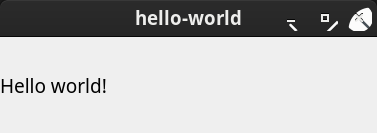
\includegraphics[height=.2\textheight]{assets/figure-hello-world}
 \end{figure}
\end{frame}

\begin{frame}[fragile]{Overview / Primer / Modify}
 If you modify an existing file:
 \begin{lstlisting}
make
\end{lstlisting}

If you add or remove files, \emph{edit hello-world.pro} and:
 \begin{lstlisting}
 qmake
 make
\end{lstlisting}

 \emph{Tip}: don't put all the code in main.cpp, create \emph{one class per entity}.
 
 \begin{columns}
  \begin{column}{0.15\textwidth}
   
\includegraphics[width=0.99\textwidth]{assets/logo-github}
  \end{column}
  \begin{column}{0.85\textwidth}
   Source code available at:
   \url{https://github.com/Unipd-Object-Oriented-Programming/hello-world}
  \end{column}
 \end{columns}
\end{frame}


%-----------------------------------------------------------------------
\section{Layout and Structure}
\begin{frame}{Layout and Structure}
 Software project simplified \emph{life-cycle}:
 \begin{figure}
  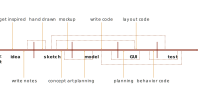
\includegraphics[width=0.95\textwidth]{assets/figure-project-plan}
 \end{figure}
\end{frame}

\begin{frame}{Layout and Structure / Idea}
 \begin{center}
  \emph{idea}
  
  it's up to you.
 \end{center}
 \vspace{2cm}
 Be sure to \emph{meet constraints}!
 
 Looking for ideas? Drop me an email at \href{mailto:marco.zanella@unipd.it}{marco.zanella@unipd.it}.
\end{frame}

\begin{frame}{Layout and Structure / Sketch}
 Start from a \emph{sketch} of your application:
 \begin{figure}
  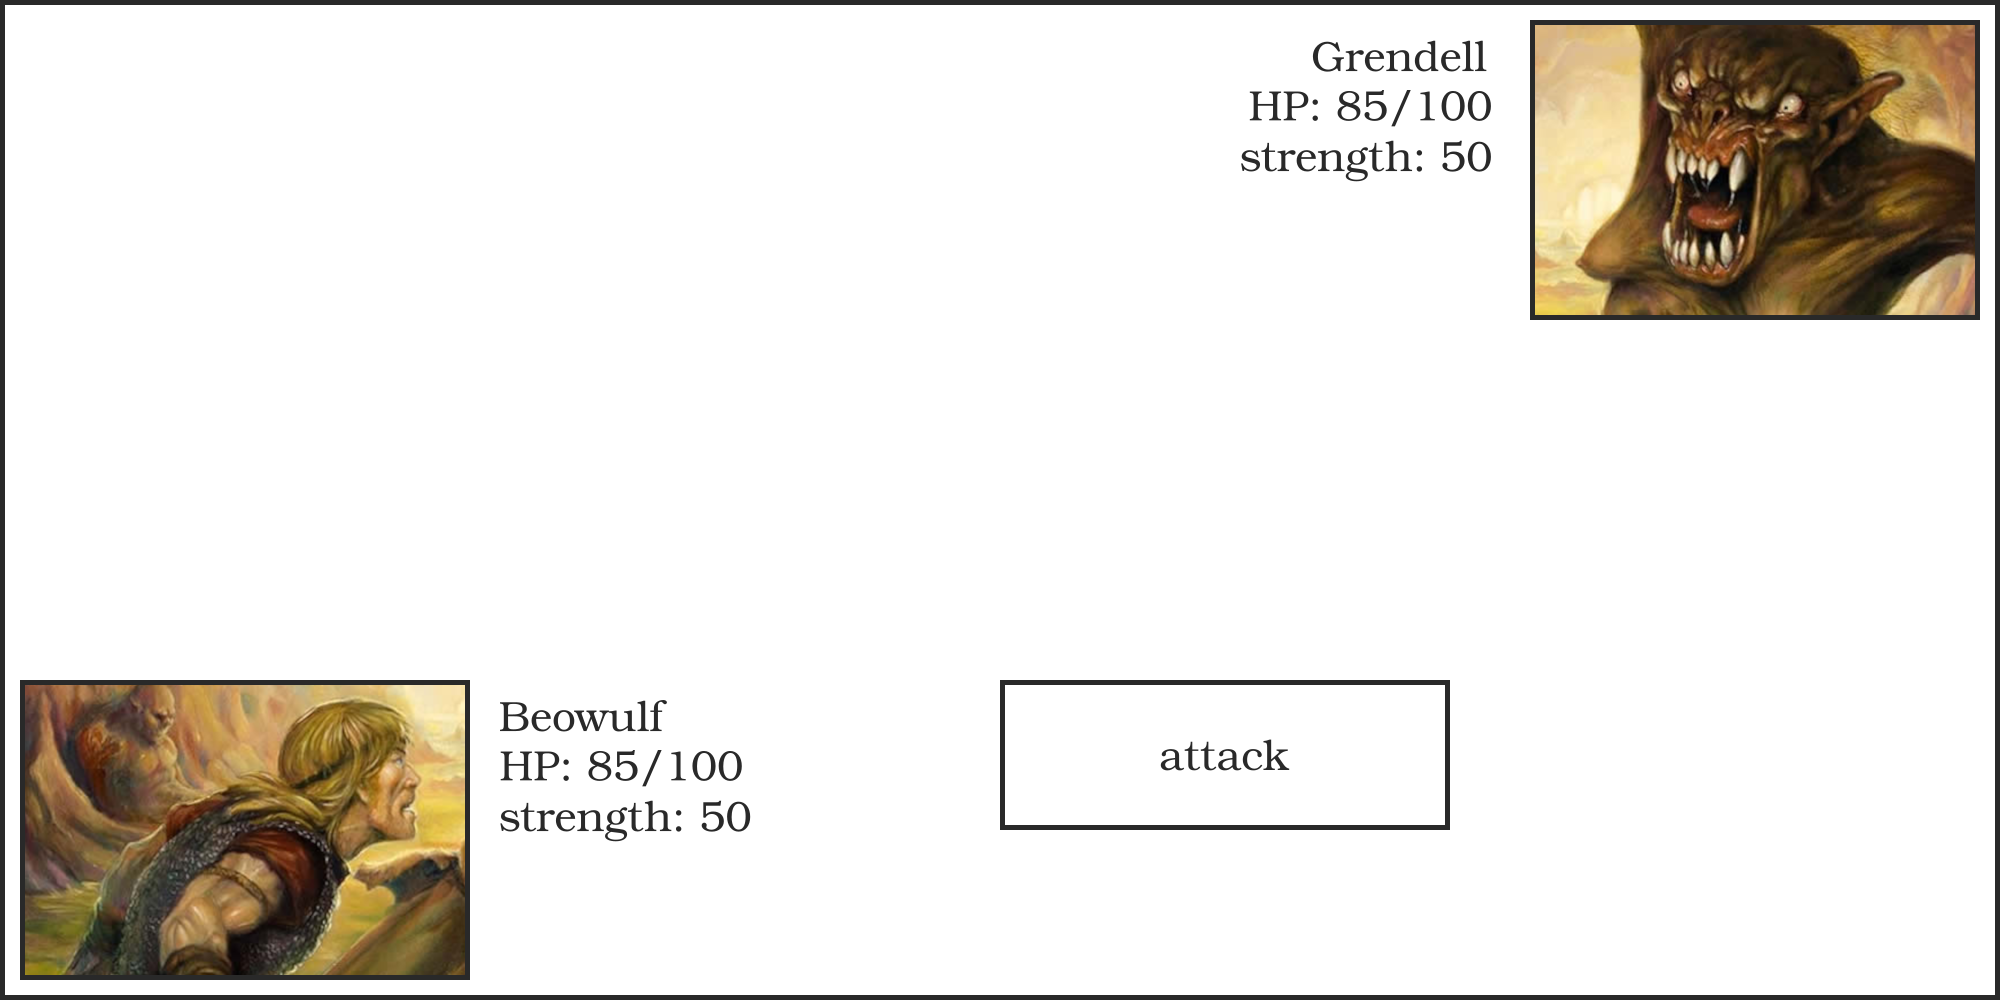
\includegraphics[width=0.95\textwidth]{assets/figure-battle-scene-1}
  \caption{Characters from "The Tale of Beowulf"}
 \end{figure}
\end{frame}

\begin{frame}{Layout and Structure / Sketch}
 Identify \emph{atomic entities}:
 \begin{figure}
  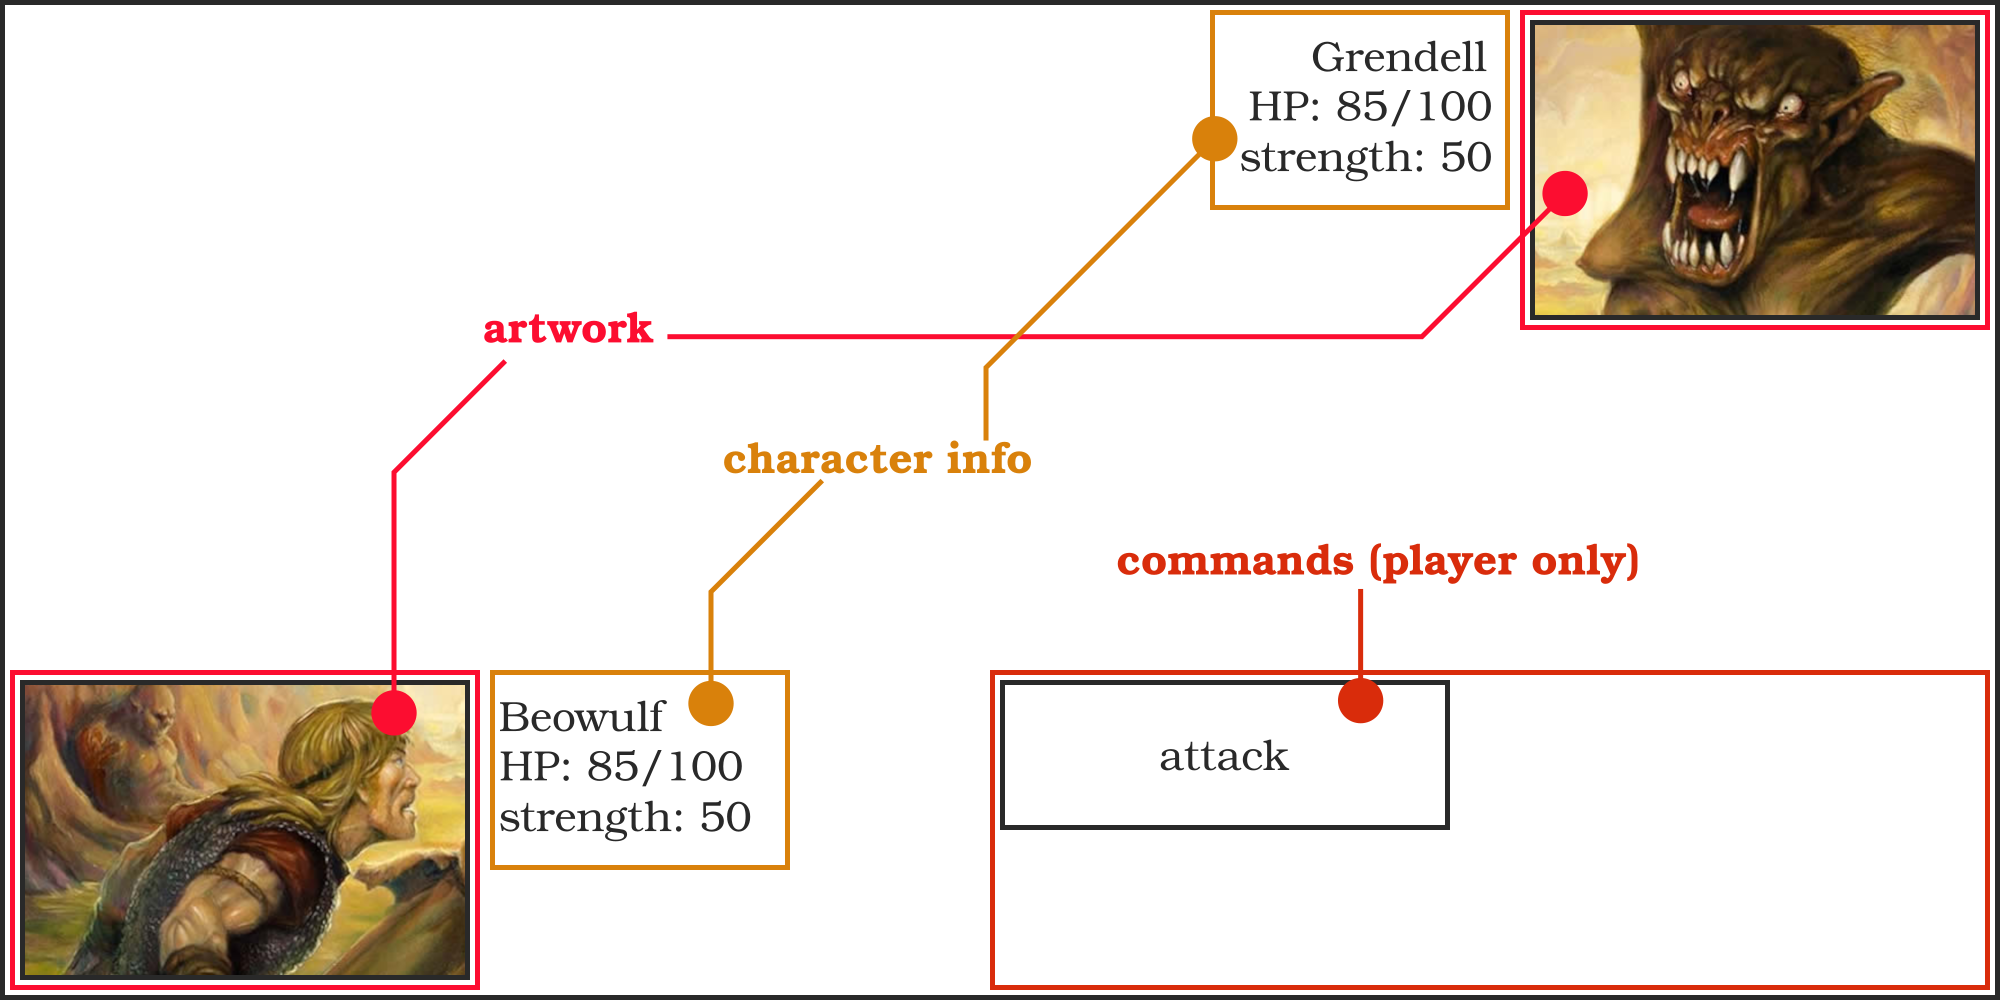
\includegraphics[width=0.95\textwidth]{assets/figure-battle-scene-2}
 \end{figure}
 those are \emph{widgets}, the backbone of your GUI.
\end{frame}

\begin{frame}{Layout and Structure / Sketch}
 Break down into \emph{rectangles}:
 \begin{figure}
  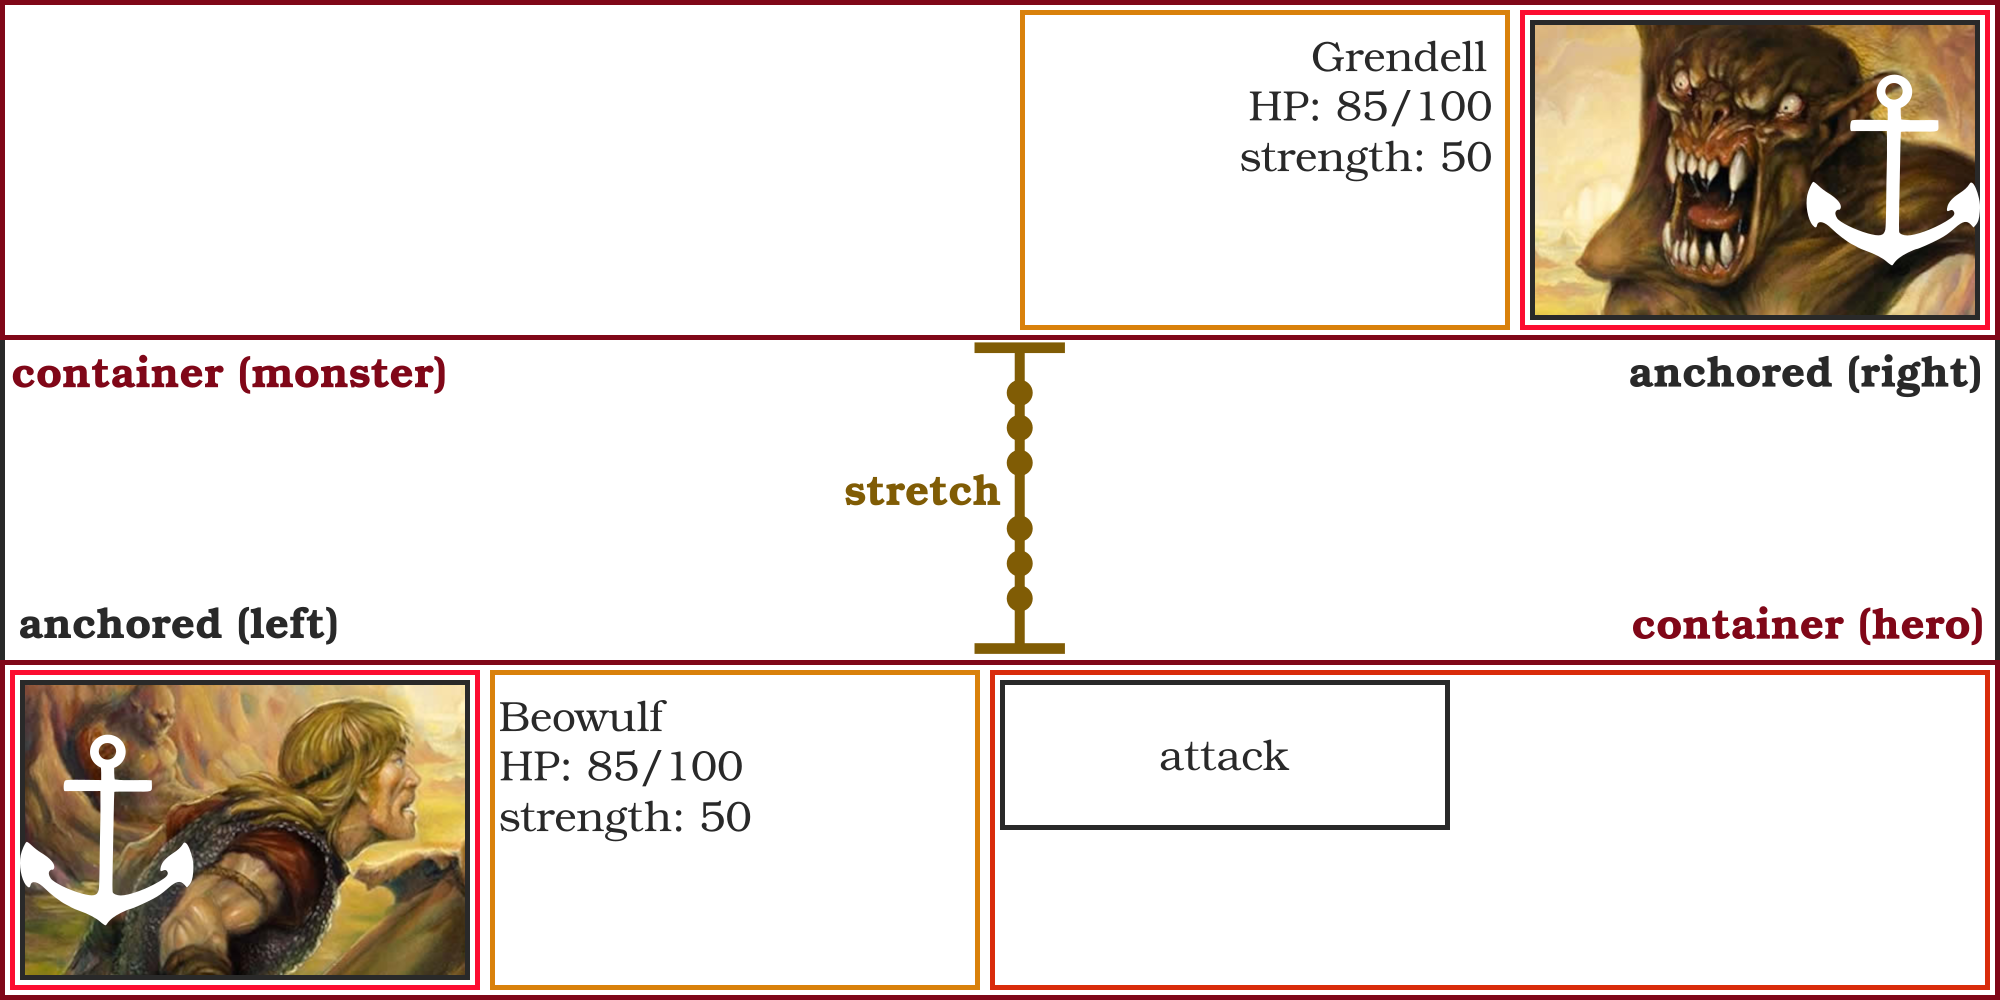
\includegraphics[width=0.95\textwidth]{assets/figure-battle-scene-3}
 \end{figure}
 those are \emph{layouts}, which organize widgets.
\end{frame}

\begin{frame}{Layout and Structure / Model}
 Plan the \emph{core model}:
 \begin{figure}
  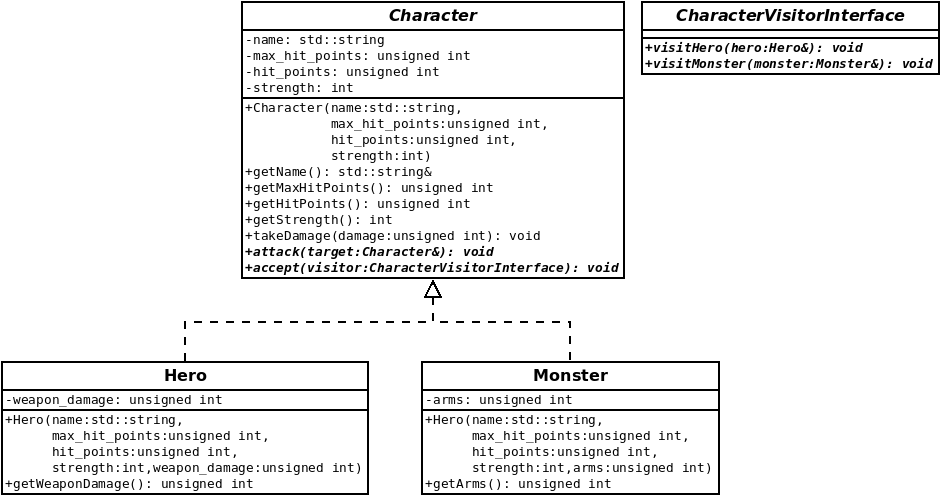
\includegraphics[height=0.65\textheight]{assets/diagram-battle-scene}
 \end{figure}
 this is unrelated from the GUI.
\end{frame}

\begin{frame}{Layout and Structure / Model}
 UML class diagrams \emph{cheatsheet}:
 \begin{itemize}
  \item one box = one class
  \item attributes and member functions
  \item colon defines types
  \item - for private fields, \# for protected, + for public
  \item arrows for inheritance
  \item italics for virtual, bold for pure virtual
 \end{itemize}
 {\scriptsize (more during your Software Engineering class)}
 
 Free-software for UML:
 \begin{center}
  
\includegraphics[height=0.1\textheight]{assets/logo-dia}\\
  Dia - \url{https://wiki.gnome.org/Apps/Dia}
 \end{center}
\end{frame}

\begin{frame}{Layout and Structure / GUI}
 Plan the \emph{GUI widgets}:
 \begin{figure}
  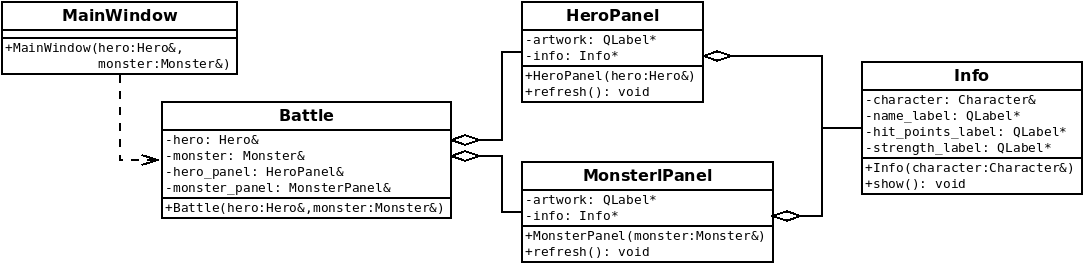
\includegraphics[width=0.95\textwidth]{assets/diagram-battle-scene-gui}
 \end{figure}
 widgets should \emph{depend on} the model.
\end{frame}

\begin{frame}[fragile]{Layout and Structure / Info}
 The \emph{Info} widget:
 \begin{columns}
  \begin{column}{0.33\textwidth}
   \fbox{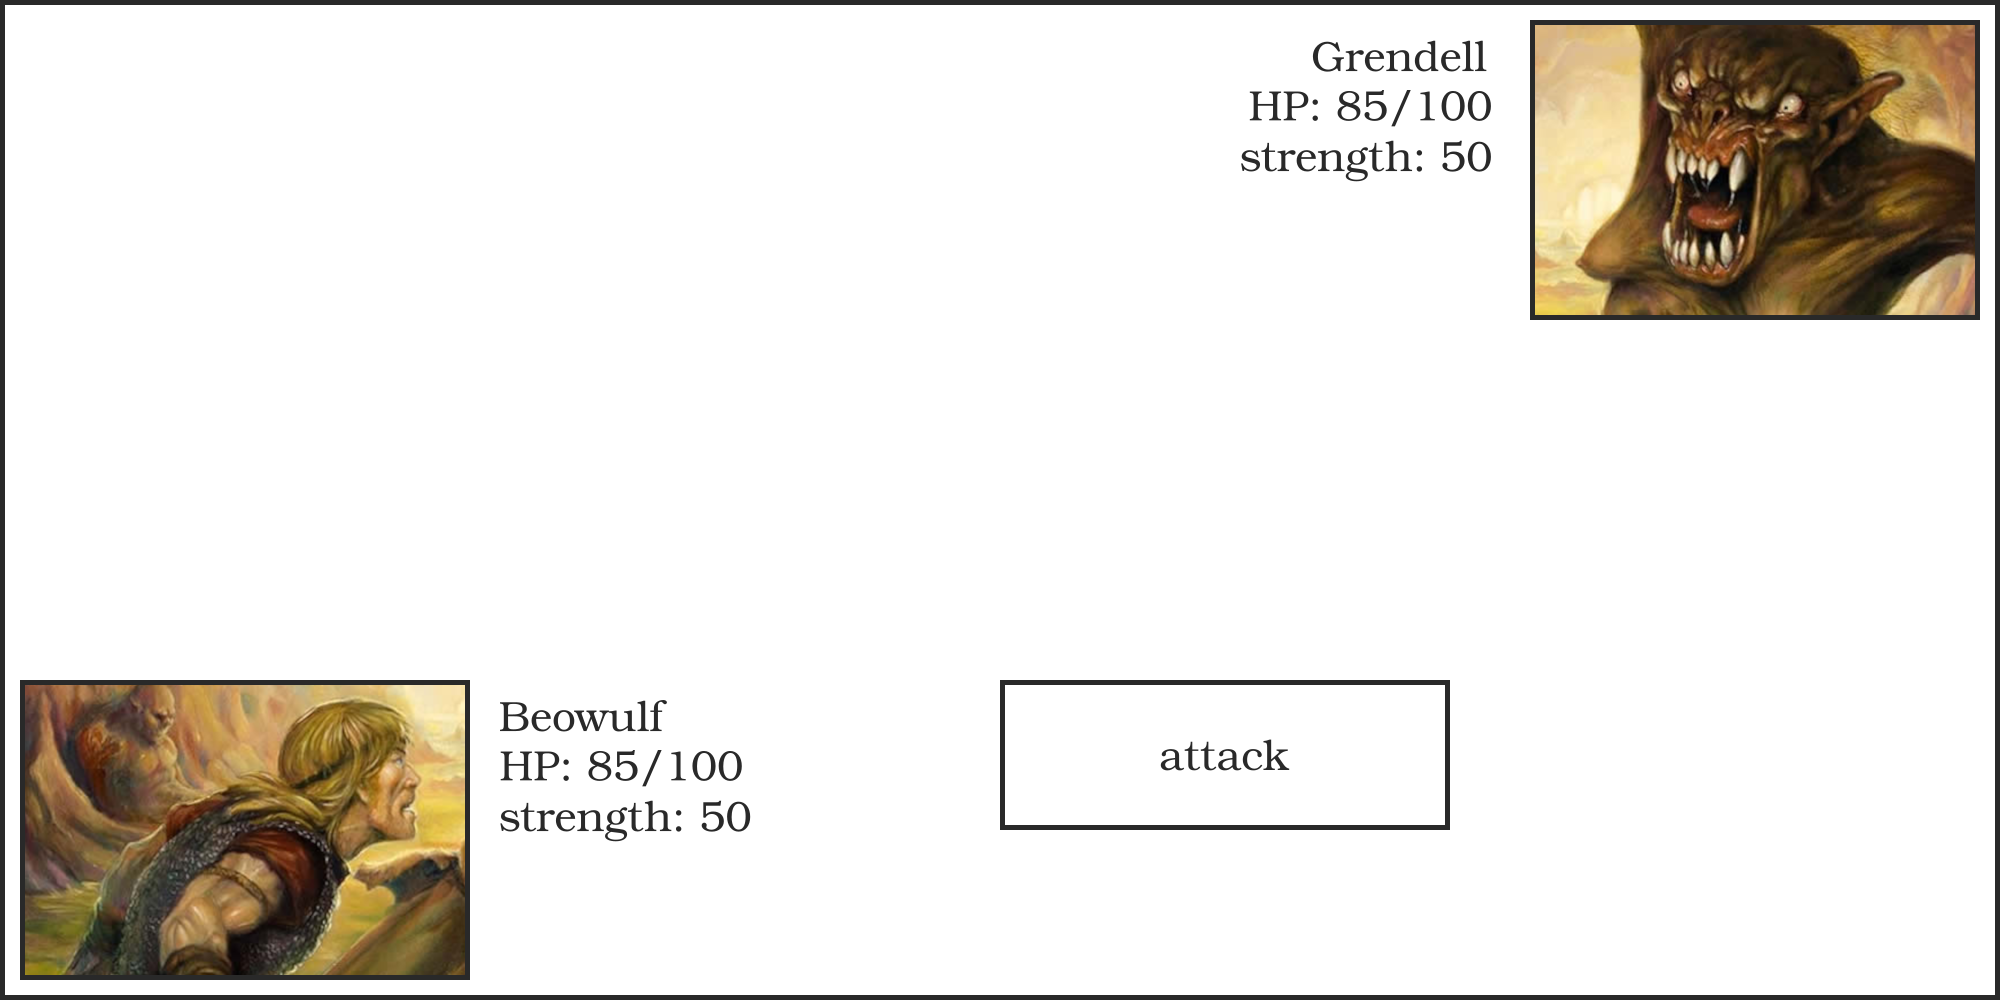
\includegraphics[trim={4.5cm 0cm 12cm 7cm},clip,width=0.90\textwidth]{assets/figure-battle-scene-1}}
  \end{column}
  \begin{column}{0.66\textwidth}
   \begin{lstlisting}[language=C++]
class Info: public QWidget {
  Q_OBJECT
 private:
  Character& character;
  QLabel* name_label;
  QLabel* hit_points_label;
  QLabel* strength_label;
 public:
  Info(Character& character, QWidget* parent = 0);
  void show();
};\end{lstlisting}
  \end{column}
 \end{columns}
 {\footnotesize inclusion of header files, namespaces, etc. omitted for brevity}
\end{frame}

\begin{frame}[fragile]{Layout and Structure / Info}
 The \emph{Info} widget:
 \begin{lstlisting}[language=C++]
Info::Info(Character& character, QWidget* parent)
  : QWidget(parent), character(character)
{
  QVBoxLayout* layout = new QVBoxLayout(this);
  layout->setAlignment(Qt::AlignLeft | Qt::AlignTop);
    
  name_label = new QLabel();
  layout->addWidget(name_label);
    
  hit_points_label = new QLabel();
  layout->addWidget(hit_points_label);
    
  strength_label = new QLabel();
  layout->addWidget(strength_label);
}
\end{lstlisting}
 {\footnotesize Constructor}
\end{frame}

\begin{frame}[fragile]{Layout and Structure / Info}
 The \emph{Info} widget:
 \begin{lstlisting}[language=C++]
void Info::show() {
  name_label->setText(QString::fromStdString(character.getName()));
  hit_points_label->setText("HP: " + QString::number(character.getHitPoints()) + "/" + QString::number(character.getMaxHitPoints()));
  strength_label->setText("Strength: " + QString::number(character.getStrength()));
}
\end{lstlisting}
 {\footnotesize Info.show()}
\end{frame}

\begin{frame}[fragile]{Layout and Structure / Info}
 The \emph{Info} widget wrap-up:
 \begin{itemize}
  \item extend \emph{QWidget}
  \item use \emph{Q\_OBJECT} macro
  \item \emph{QVBoxLayout} to arrange widgets vertically
  \item mind \emph{alignment}
  \item use \emph{QString}
 \end{itemize}
\end{frame}

\begin{frame}[fragile]{Layout and Structure / HeroPanel}
 The \emph{HeroPanel} widget:
 \begin{center}
  \fbox{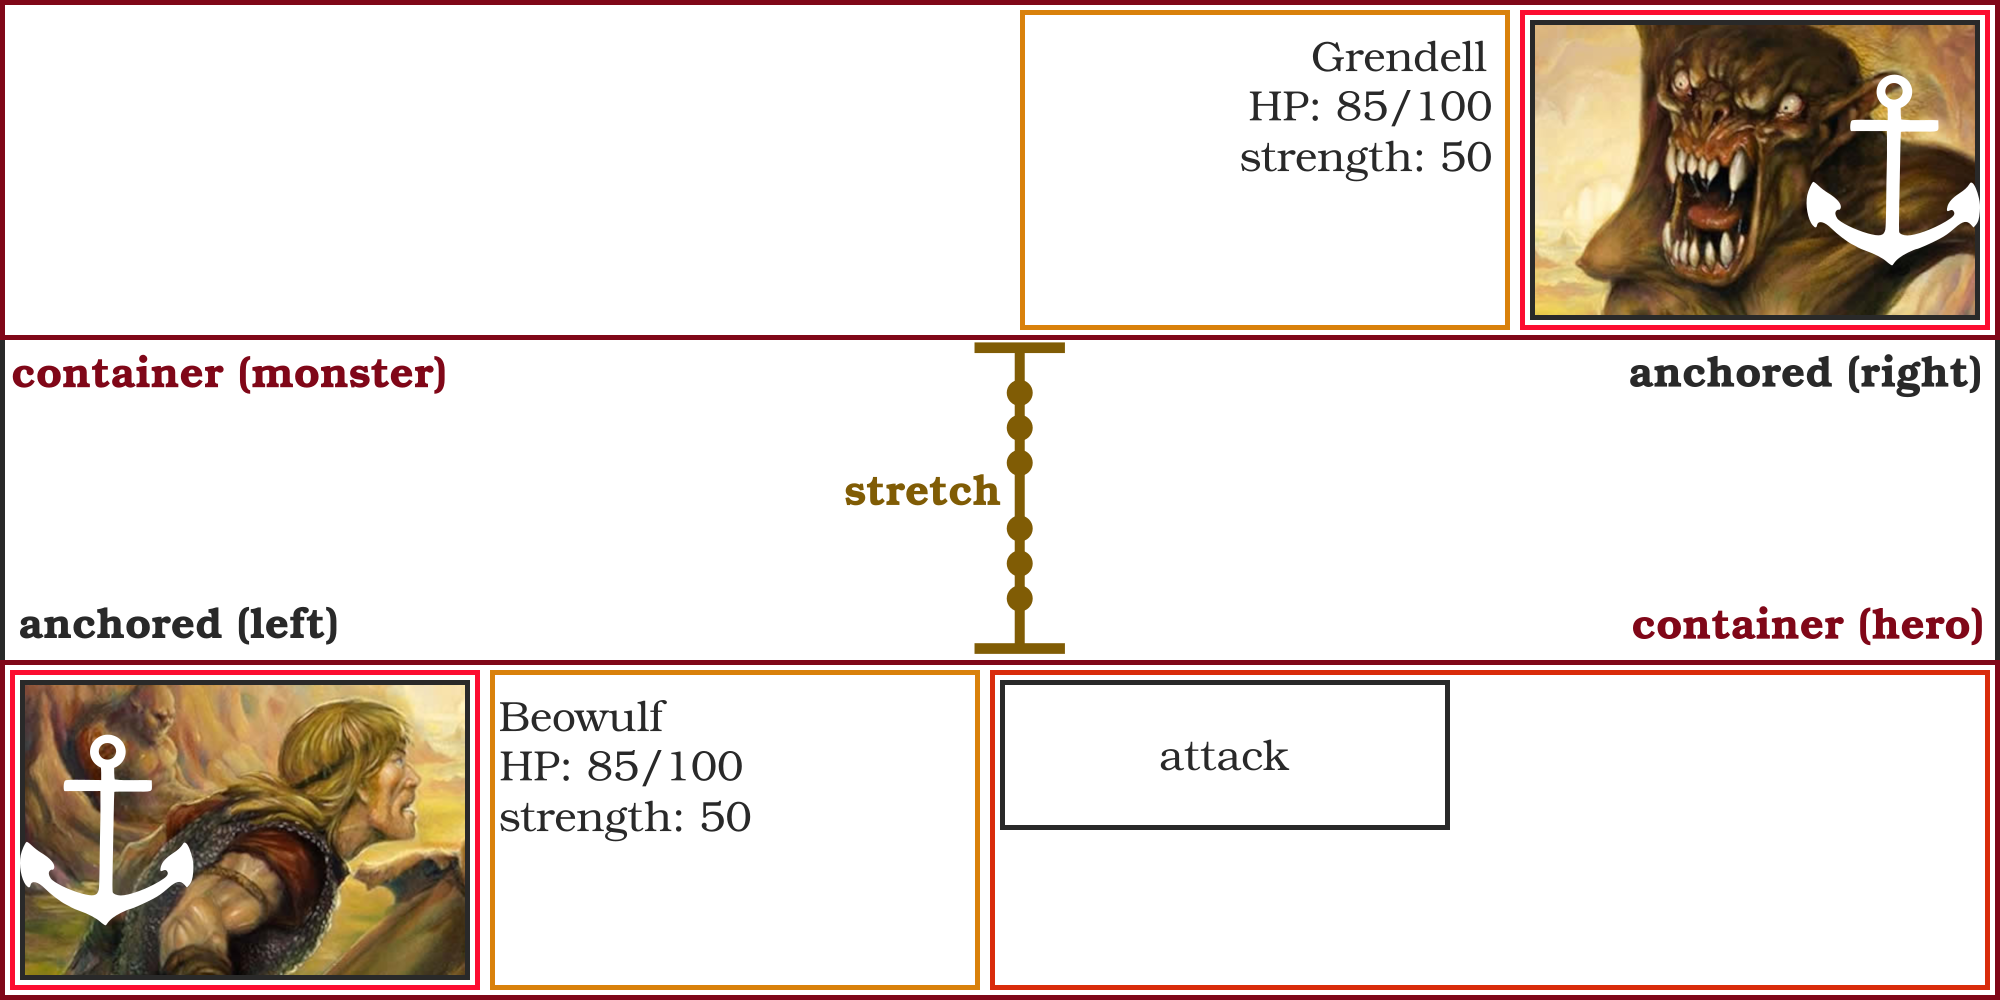
\includegraphics[trim={0cm 0cm 0cm 6.5cm},clip,height=0.2\textheight]{assets/figure-battle-scene-3}}
 \end{center}
 \begin{lstlisting}[language=C++]
class HeroPanel: public QWidget {
  Q_OBJECT
 private:
  QLabel* artwork;
  Info* info;
 public:
  HeroPanel(Game::Hero& hero, QWidget* parent = 0);
  void refresh();
};
\end{lstlisting}
\end{frame}

\begin{frame}[fragile]{Layout and Structure / HeroPanel}
 The \emph{HeroPanel} widget:
 \begin{lstlisting}[language=C++]
HeroPanel::HeroPanel(Game::Hero& hero, QWidget* parent)
  : QWidget(parent)
{
  QHBoxLayout* layout = new QHBoxLayout(this);
  layout->setAlignment(Qt::AlignLeft | Qt::AlignTop);

  QPixmap image(":assets/" + QString::fromStdString(hero.getName()) + ".png");
  artwork = new QLabel();
  artwork->setPixmap(image.scaledToHeight(256));
  layout->addWidget(artwork);

  info = new Info(hero);
  info->show();
  layout->addWidget(info);
\end{lstlisting}
{\footnotesize continues next slide}
\end{frame}

\begin{frame}[fragile]{Layout and Structure / HeroPanel}
 The \emph{HeroPanel} widget:
 \begin{lstlisting}[language=C++]
  // Adds commands
  QGridLayout* commands = new QGridLayout();
  layout->addLayout(commands);

  QPushButton* attack = new QPushButton("attack");
  commands->addWidget(attack, 0, 0, 1, 1);

  QPushButton* items = new QPushButton("items");
  items->setEnabled(false);
  commands->addWidget(items, 0, 1, 1, 1);

  QPushButton* skills = new QPushButton("skills");
  skills->setEnabled(false);
  commands->addWidget(skills, 1, 0, 1, 1);
}

void HeroPanel::refresh() { info->show(); }
\end{lstlisting}
\end{frame}

\begin{frame}[fragile]{Layout and Structure / HeroPanel}
 The \emph{HeroPanel} widget wrap-up:
 \begin{itemize}
  \item \emph{QHBoxLayout} to arrange widgets horizontally
  \item \emph{QPixmap} and \emph{QLabel} for images
  \item \emph{QGridLayout} for a grid of widgets
  \item commands as \emph{QPushButtom}
  \item member function to encapsulate \emph{refresh} logic
 \end{itemize}
 
 The \emph{MonsterPanel} is analogous without buttons.
\end{frame}

\begin{frame}[fragile]{Layout and Structure / Battle}
 The \emph{Battle} widget:
 \begin{lstlisting}[language=C++]
class Battle: public QWidget {
  Q_OBJECT

 private:
  Game::Hero& hero;
  Game::Monster& monster;
  HeroPanel* hero_panel;
  MonsterPanel* monster_panel;

 public:
  Battle(Game::Hero& hero, Game::Monster& monster, QWidget* parent = 0);
  
 public slots:
  void playerAttacks();
};
\end{lstlisting}
\end{frame}

\begin{frame}[fragile]{Layout and Structure / Battle}
 The \emph{Battle} widget:
 \begin{lstlisting}[language=C++]
Battle::Battle(Game::Hero& hero, Game::Monster& monster, QWidget* parent)
  : QWidget(parent), hero(hero), monster(monster)
{
  QVBoxLayout* layout = new QVBoxLayout(this);

  monster_panel = new MonsterPanel(monster);
  layout->addWidget(monster_panel);

  layout->addStretch();

  hero_panel = new HeroPanel(hero);
  layout->addWidget(hero_panel);
}
\end{lstlisting}
\end{frame}

\begin{frame}[fragile]{Layout and Structure / Battle}
 The \emph{Battle} widget:
 \begin{lstlisting}[language=C++]
void Battle::playerAttacks() {
  hero.attack(monster);
  monster_panel->refresh();
  monster.attack(hero);
  hero_panel->refresh();
}
\end{lstlisting}

 The \emph{Battle} widget wrap-up:
 \begin{itemize}
  \item \emph{QHVoxLayout} to arrange widgets vertically
  \item work by \emph{aggregating} other widgets
  \item expose member functions to \emph{react to events}
 \end{itemize}
\end{frame}

\begin{frame}[fragile]{Layout and Structure / MainWindow}
 The \emph{MainWindow} window:
 \begin{lstlisting}[language=C++]
class MainWindow: public QMainWindow {
  Q_OBJECT
 public:
  MainWindow(Game::Hero& hero, Game::Monster& monster);
};
\end{lstlisting}
 \begin{lstlisting}[language=C++]
MainWindow::MainWindow(Game::Hero& hero, Game::Monster& monster) {
  Battle* battle_scene = new Battle(hero, monster);
  setCentralWidget(battle_scene);
}
\end{lstlisting}

 The \emph{MainWindow} window wrap-up:
 \begin{itemize}
  \item extend \emph{QMainWindow}
  \item use \emph{setCentralWidget}
 \end{itemize}
\end{frame}

\begin{frame}[fragile]{Layout and Structure / main}
 The \emph{main} function:
 \begin{lstlisting}[language=C++]
int main(int argc, char *argv[]) {
  QApplication app(argc, argv);
  Game::Hero beowulf("Beowulf", 100, 100, 50, 10);
  Game::Monster grendel("Grendel", 250, 250, 5, 2);
  Game::View::MainWindow main_window(beowulf, grendel);
  main_window.resize(1024, 512);
  main_window.show();
  return app.exec();
}
\end{lstlisting}

 \begin{columns}
  \begin{column}{0.15\textwidth}
   
\includegraphics[width=0.99\textwidth]{assets/logo-github}
  \end{column}
  \begin{column}{0.85\textwidth}
   Source code available at:
   \url{https://github.com/Unipd-Object-Oriented-Programming/game}
  \end{column}
 \end{columns}
\end{frame}

\begin{frame}[fragile]{Layout and Structure / Wrap-Up}
 \begin{columns}
  \begin{column}{0.55\textwidth}
    \begin{forest}
     for tree={
       font=\ttfamily,
       grow'=0,
       child anchor=west,
       parent anchor=south,
       anchor=west,
       calign=first,
       edge path={
         \noexpand\path [draw, \forestoption{edge}]
         (!u.south west) +(7.5pt,0) |- node[fill,inner sep=1.25pt] {} (.child anchor)\forestoption{edge label};
       },
       before typesetting nodes={
         if n=1
           {insert before={[,phantom]}}
           {}
       },
       fit=band,
       before computing xy={l=15pt},
     }
   [MainWindow
     [Battle
       [VBoxLayout
         [HeroPanel
           [HBoxLayout
             [QLabel (artwork)]
             [Info...]
             [QGridLayout...]
           ]
         ]
         [MonsterPanel
           [HBoxLayout
             [...]
           ]
         ]
       ]
     ]
   ]
   \end{forest}
  \end{column}
  \begin{column}{0.41\textwidth}
   Widgets:
   \begin{itemize}
    \item organized in a \emph{tree}
    \item parent - child relation
    \item work by \emph{composition}
    \item automatic \emph{destruction}
   \end{itemize}
   
   Layouts:
   \begin{itemize}
    \item \emph{contain} widgets
    \item \emph{are contained} in widgets
    \item \emph{arrange} content
    \item mind \emph{alignment}
   \end{itemize}
  \end{column}
 \end{columns}
\end{frame}


%-----------------------------------------------------------------------
\section{Behavior}
\begin{frame}{Behavior}
 Do \emph{something} in response to an \emph{event}:
 \begin{figure}
  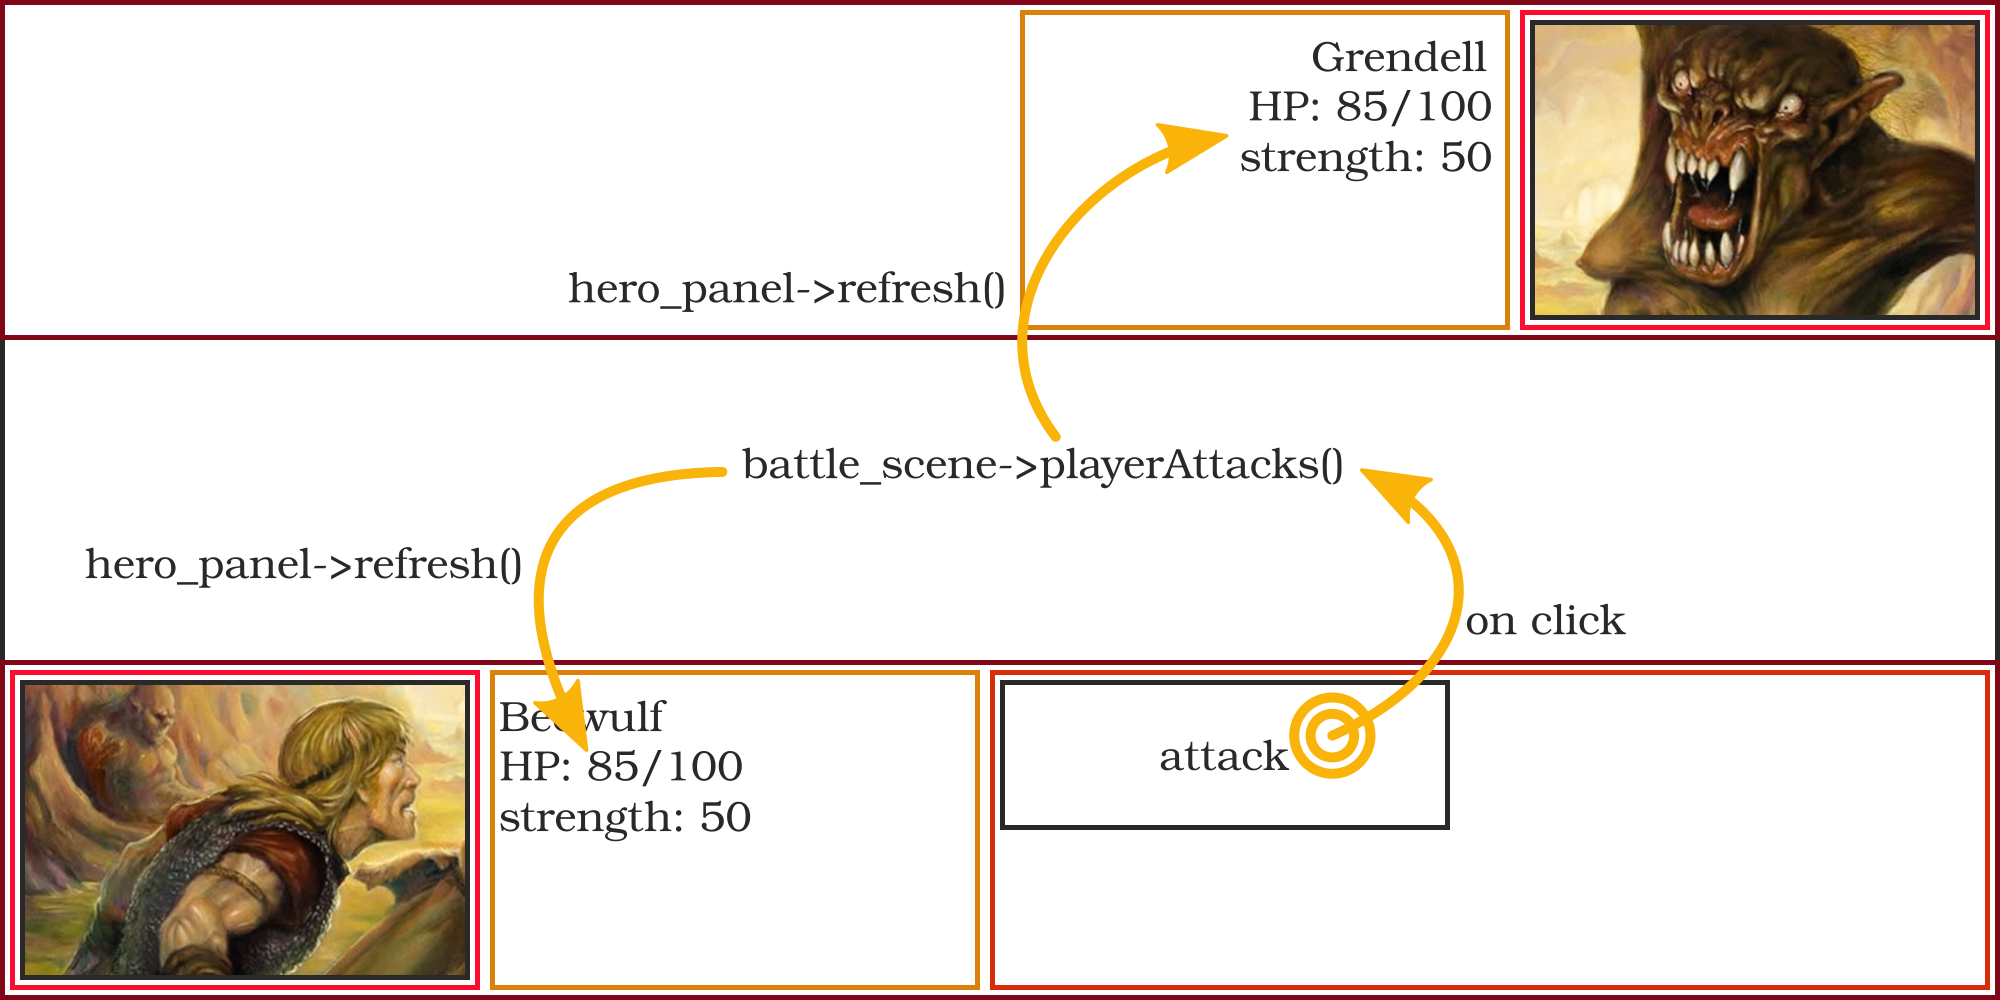
\includegraphics[width=0.95\textwidth]{assets/figure-battle-scene-4}
 \end{figure}
 run code \emph{on click}.
\end{frame}

\begin{frame}{Behavior / Event Driven Programming}
 An informal notation for events:
 \begin{figure}
  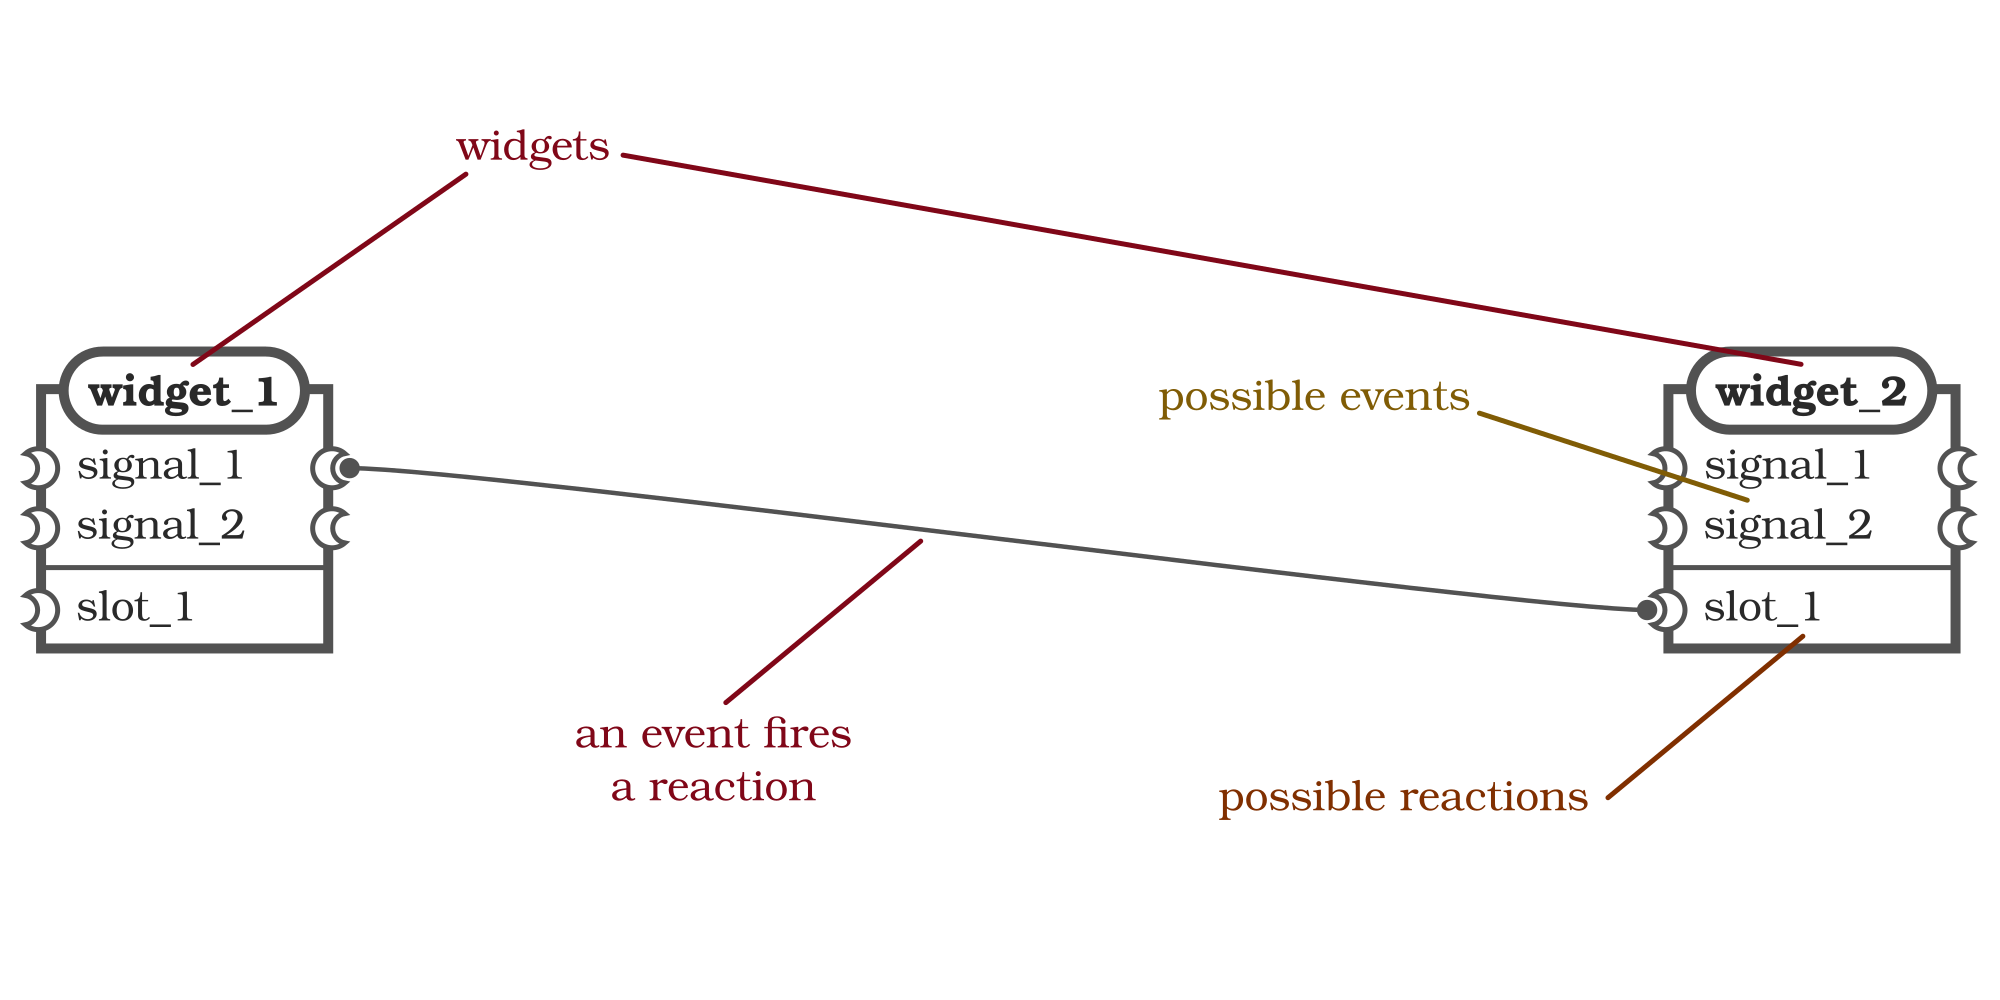
\includegraphics[width=0.95\textwidth]{assets/event-driven-programming-1}
 \end{figure}
 Event Driven Programming relies on \emph{events} and \emph{slots}.
\end{frame}

\begin{frame}{Behavior / Event Driven Programming}
 Signals can connect to other signals:
 \begin{figure}
  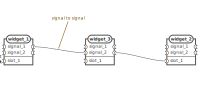
\includegraphics[width=0.95\textwidth]{assets/event-driven-programming-2}
 \end{figure}
 Informally known as \emph{signal relay}.
\end{frame}

\begin{frame}{Behavior / Event Driven Programming}
 Our game:
 \begin{figure}
  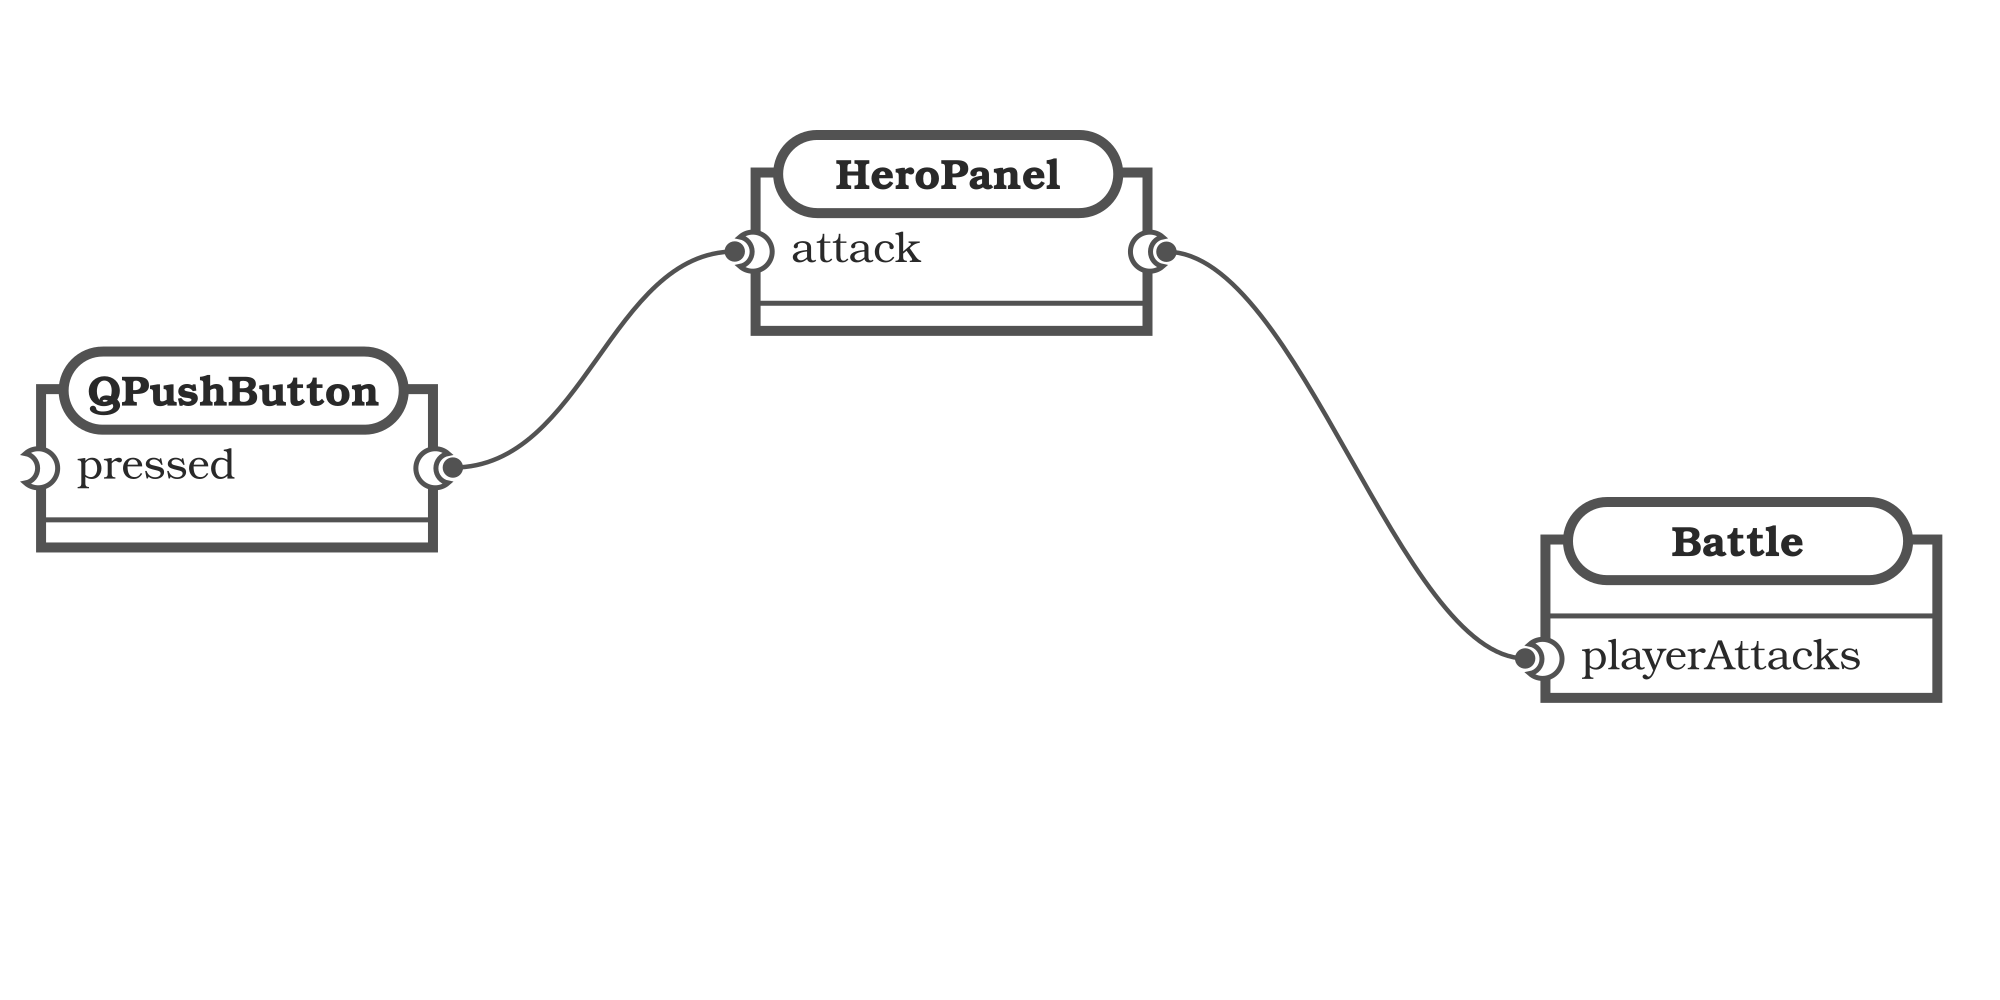
\includegraphics[width=0.95\textwidth]{assets/event-driven-programming-3}
 \end{figure}
 \emph{Battle::playerAttacks} handles the event.
\end{frame}

\begin{frame}[fragile]{Behavior / Event Driven Programming}
 Signals \emph{declared} in header file:
 \begin{lstlisting}[language=C++]
class HeroPanel: public QWidget {
  Q_OBJECT
 private:
  QLabel* artwork;
  Info* info;
 public:
  HeroPanel(Game::Hero& hero, QWidget* parent = 0);
  void refresh();
  
 signals:
  void attack();
};
\end{lstlisting}
 Signals look like member functions, but \emph{are not implemented}.
\end{frame}

\begin{frame}[fragile]{Behavior / Event Driven Programming}
 Slots \emph{declared} in header file:
 \begin{lstlisting}[language=C++]
class Battle: public QWidget {
  Q_OBJECT

 private:
  Game::Hero& hero;
  Game::Monster& monster;
  HeroPanel* hero_panel;
  MonsterPanel* monster_panel;

 public:
  Battle(Game::Hero& hero, Game::Monster& monster, QWidget* parent = 0);
  
 public slots:
  void playerAttacks();
};
\end{lstlisting}
 Slots are member functions, and \emph{must be implemented}.
\end{frame}

\begin{frame}[fragile]{Behavior / Event Driven Programming}
 Signal \emph{connected} to slot:
 \begin{lstlisting}[language=C++]
Battle::Battle(Game::Hero& hero, Game::Monster& monster, QWidget* parent)
  : QWidget(parent), hero(hero), monster(monster)
{
  QVBoxLayout* layout = new QVBoxLayout(this);

  monster_panel = new MonsterPanel(monster);
  layout->addWidget(monster_panel);

  layout->addStretch();

  hero_panel = new HeroPanel(hero);
  layout->addWidget(hero_panel);
  connect(hero_panel, &HeroPanel::attack, this, &Battle::playerAttacks);
}
\end{lstlisting}
 \texttt{connect(source\_widget, signal, destination\_widget, slot);}
\end{frame}

\begin{frame}[fragile]{Behavior / Event Driven Programming}
 Signal \emph{connected} to signal:
 \begin{lstlisting}[language=C++]
HeroPanel::HeroPanel(Game::Hero& hero, QWidget* parent)
  : QWidget(parent)
{
  ...    
  // Adds commands
  QGridLayout* commands = new QGridLayout();
  layout->addLayout(commands);

  QPushButton* attack = new QPushButton("attack");
  commands->addWidget(attack, 0, 0, 1, 1);
  connect(attack, &QPushButton::pressed, this, &HeroPanel::attack);
  ...
}
\end{lstlisting}
 \texttt{connect(source\_widget, signal, destination\_widget, signal);}
\end{frame}

\begin{frame}{Behavior / Event Driven Programming}
 More about signals and slots:
 \begin{figure}
  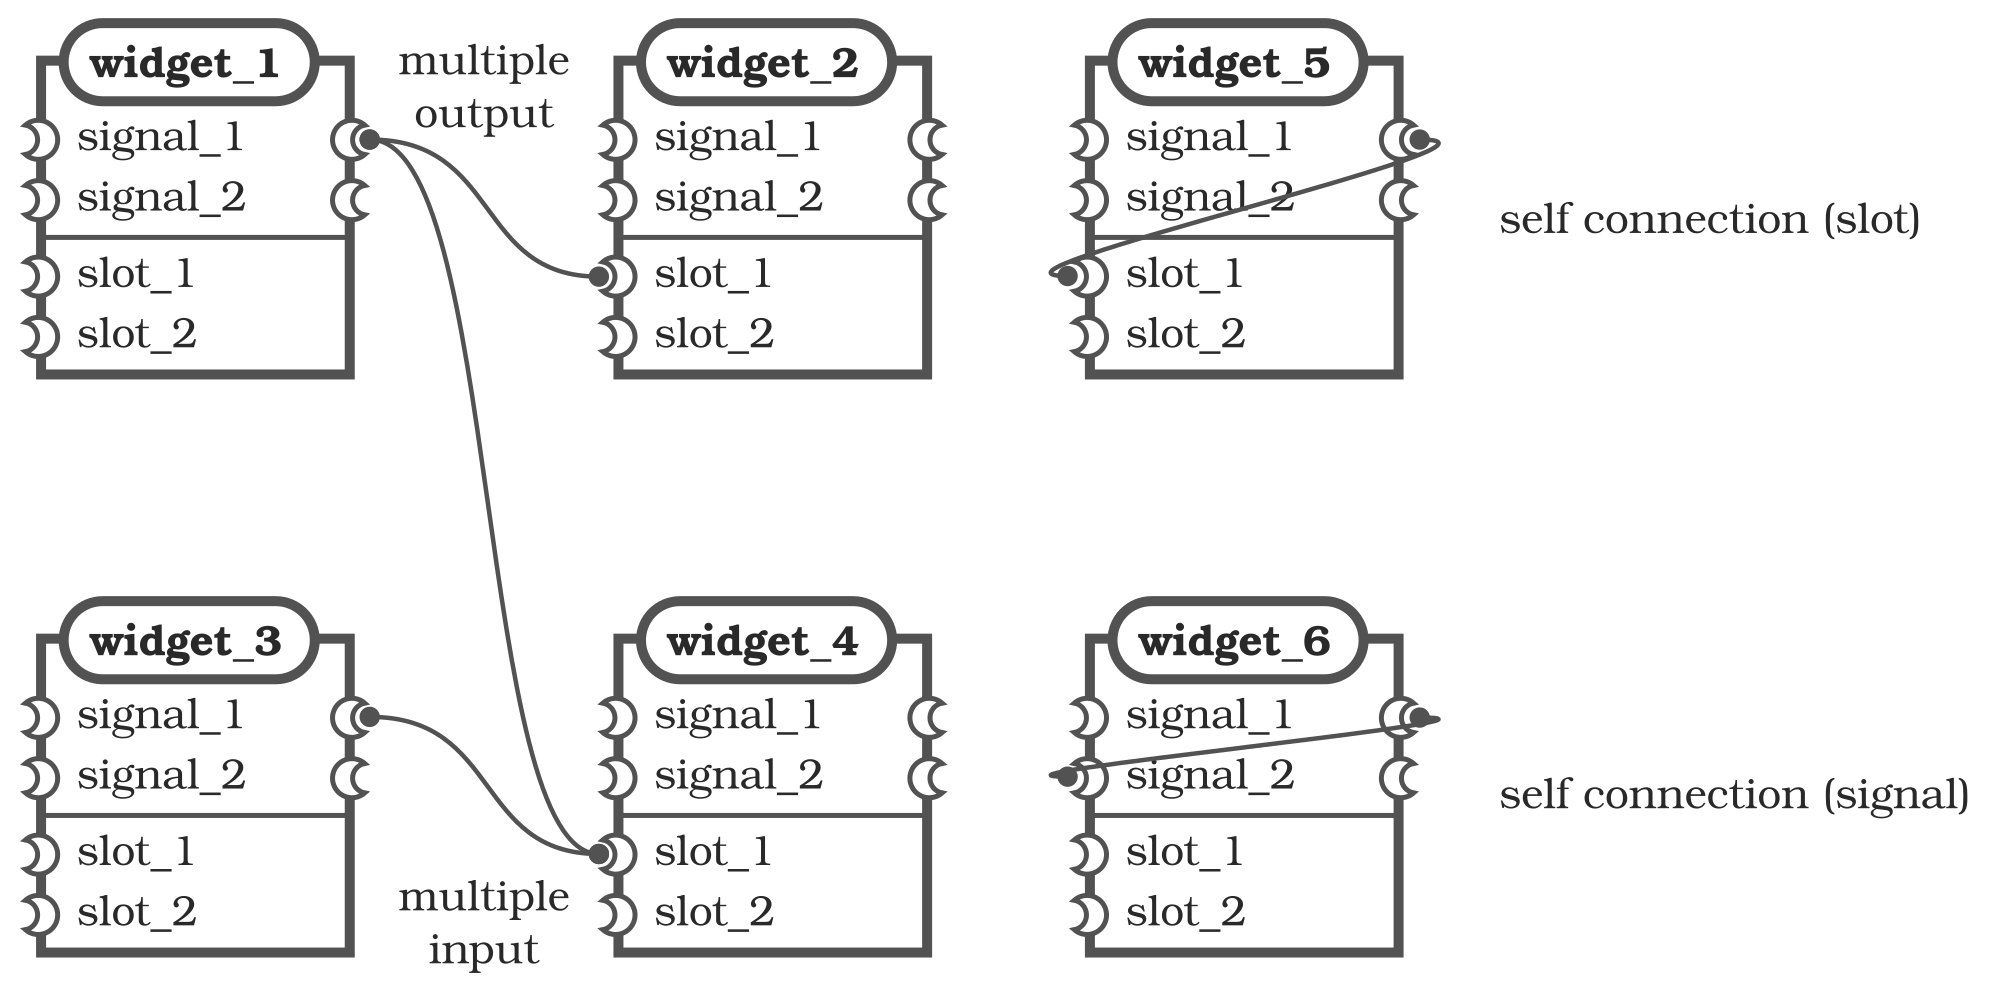
\includegraphics[width=0.95\textwidth]{assets/event-driven-programming-4}
 \end{figure}
 Everything can be combined.
\end{frame}

\begin{frame}{Behavior / Event Driven Programming}
 Signals and slots can have \emph{types}:
 \begin{figure}
  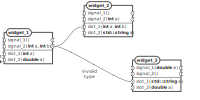
\includegraphics[width=0.95\textwidth]{assets/event-driven-programming-5}
 \end{figure}
 Different types cannot connect.
\end{frame}

\begin{frame}{Behavior / Visual Scripting}
 Other frameworks using similar ideas:
 \begin{center}
  \begin{figure}
   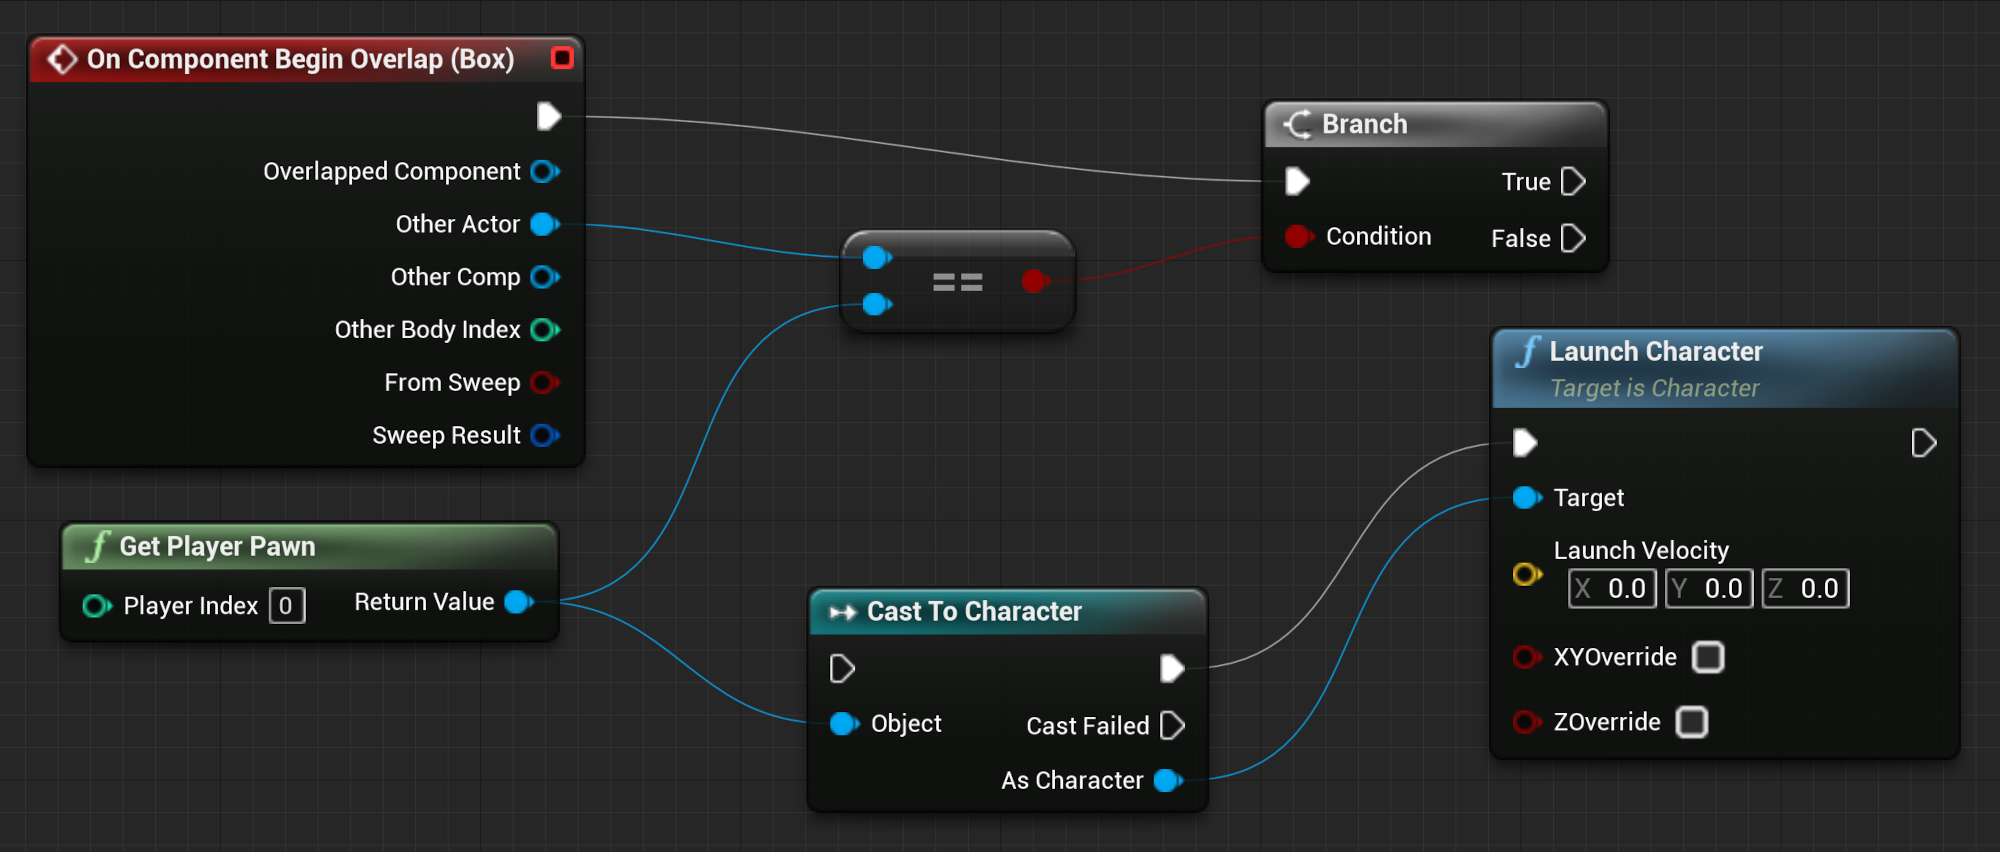
\includegraphics[width=0.95\textwidth]{assets/figure-visual-script-unreal}
  \end{figure}
  \href{https://www.unrealengine.com/en-US}{Unreal Engine} blueprints
 \end{center}
\end{frame}

\begin{frame}{Behavior / Visual Scripting}
 Other frameworks using similar ideas:
 \begin{center}
  \begin{figure}
   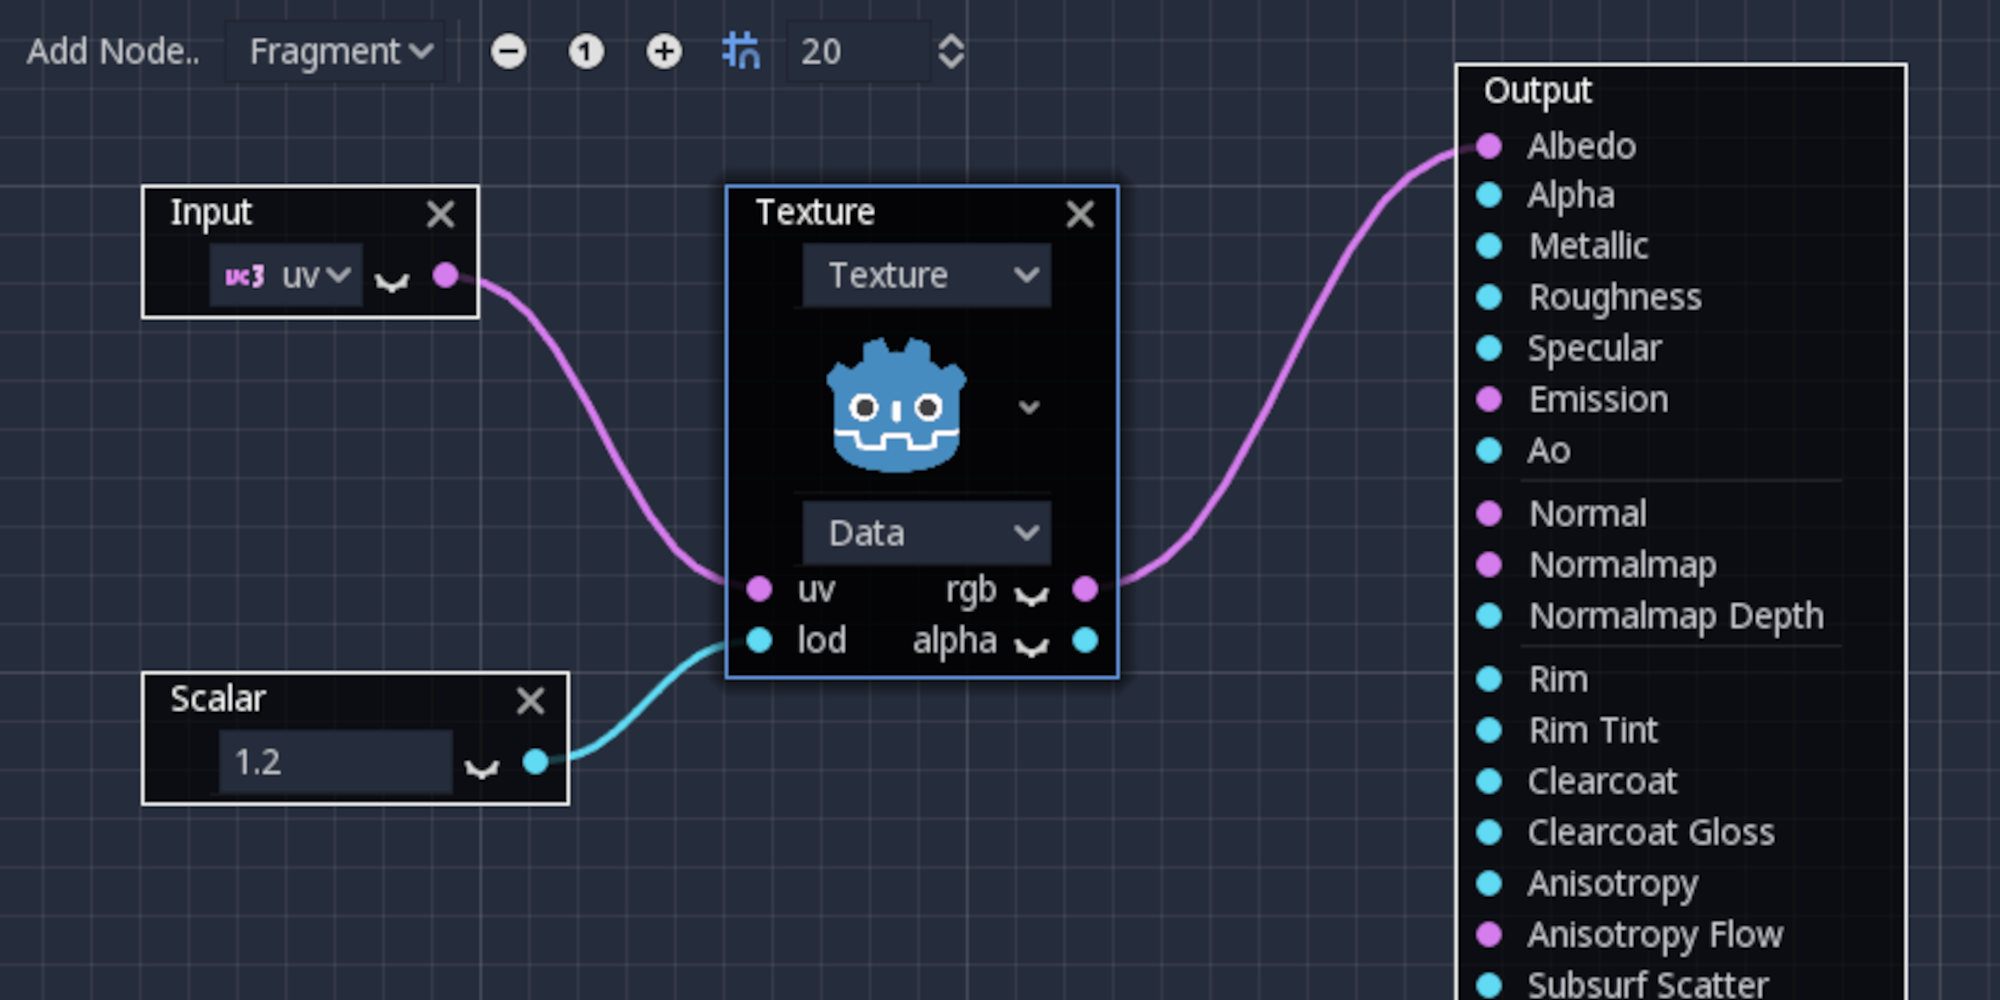
\includegraphics[width=0.95\textwidth]{assets/figure-visual-script-godot}
  \end{figure}
  \href{https://godotengine.org/}{Godot Engine}
 \end{center}
\end{frame}


%-----------------------------------------------------------------------
\section{Polymorphism}
\begin{frame}{Polymorphism}
 Literally \emph{multiple shapes}:
 \begin{figure}
  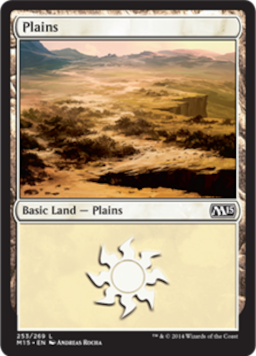
\includegraphics[width=0.13\textwidth]{assets/figure-magic-land}
  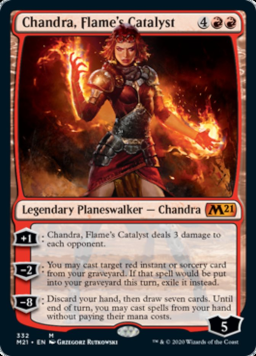
\includegraphics[width=0.13\textwidth]{assets/figure-magic-creature}
  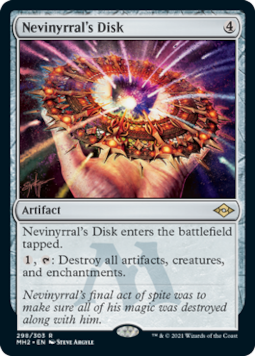
\includegraphics[width=0.13\textwidth]{assets/figure-magic-artifact}
  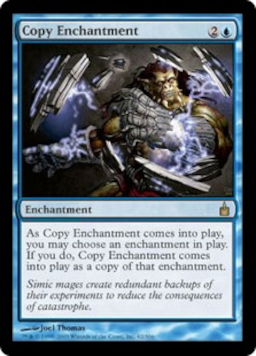
\includegraphics[width=0.13\textwidth]{assets/figure-magic-enchantment}
  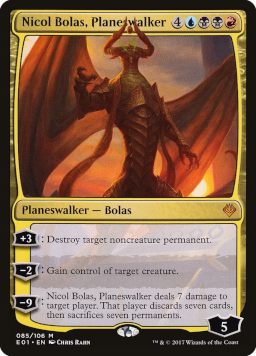
\includegraphics[width=0.13\textwidth]{assets/figure-magic-planeswalker}
  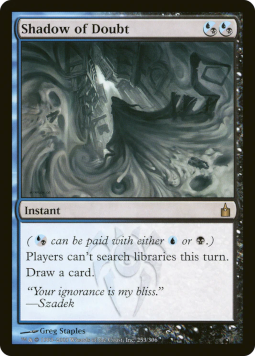
\includegraphics[width=0.13\textwidth]{assets/figure-magic-instant}
  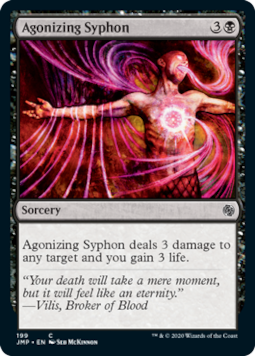
\includegraphics[width=0.13\textwidth]{assets/figure-magic-sorcery}
  \caption{Magic: the Gathering Types of Cards}
 \end{figure}
 An \emph{abstract type} varying its behavior depending on \emph{concrete type}.
\end{frame}

\begin{frame}{Polymorphism / Visitor}
 How to \emph{show} different cards?
 \begin{figure}
  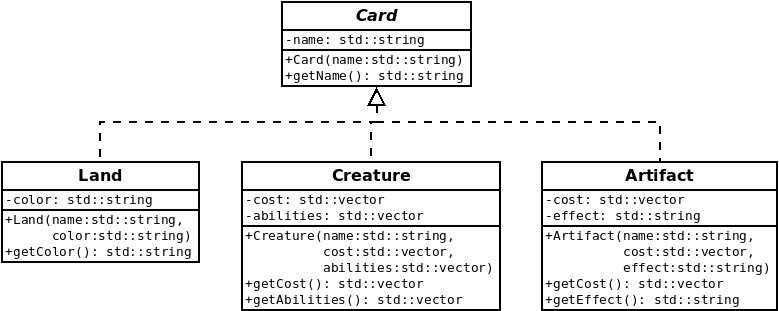
\includegraphics[width=0.80\textwidth]{assets/diagram-cards}
 \end{figure}
 Recurring problem: showing \emph{different subtypes}.
\end{frame}

\begin{frame}{Polymorphism / Visitor}
 How to \emph{show} different details for creatures?
 \begin{figure}
  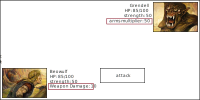
\includegraphics[width=0.95\textwidth]{assets/figure-battle-scene-5}
 \end{figure}
 Recurring problem: showing \emph{different subtypes}.
\end{frame}

\begin{frame}{Polymorphism / Visitor}
 Common \emph{wrong} or \emph{non optimal} approaches:
 \begin{itemize}
  \item \texttt{std::string Character::getContent()} member function
  \item \texttt{QWidget* Character::render()} member function
  \item RTTI / dynamic cast / typeid
  \item \texttt{std::string Character::getType()} member function
 \end{itemize}
 May work for tiny projects, but \emph{likely to fail} in bigger ones.
\end{frame}

\begin{frame}[fragile]{Polymorphism / Visitor}
 Common \emph{wrong} or \emph{non optimal} approaches:
 
 \begin{center}
  \texttt{std::string Character::getContent()} member function
 \end{center}
 
 \begin{columns}
  \begin{column}{0.45\textwidth}
   \begin{lstlisting}[language=C++]
class Character {
 public:
  virtual std::string getContent() = 0;
};
\end{lstlisting}
  \end{column}
  \begin{column}{0.55\textwidth}
   \begin{lstlisting}[language=C++]
std::string Hero::getContent() {
  return "Weapon Damage " + std::string(weapon_damage);
};

std::string Monster::getContent() {
  return "Arms Multiplier " + std::string(arms);
};
\end{lstlisting}
  \end{column}
 \end{columns}
 Works when difference is \emph{merely a string}.
\end{frame}

\begin{frame}[fragile]{Polymorphism / Visitor}
 Common \emph{wrong} or \emph{non optimal} approaches:
 
 \begin{center}
  \texttt{std::string Character::getContent()} member function
 \end{center}
 
 \begin{figure}
  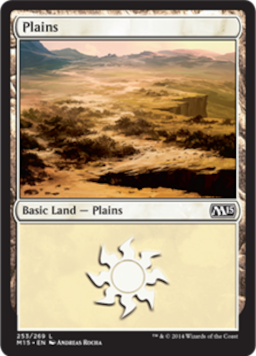
\includegraphics[width=0.25\textwidth]{assets/figure-magic-land}
  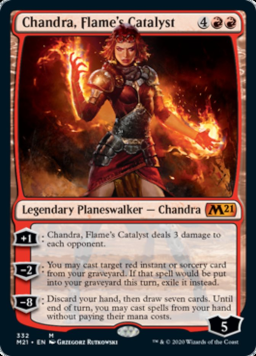
\includegraphics[width=0.25\textwidth]{assets/figure-magic-creature}
  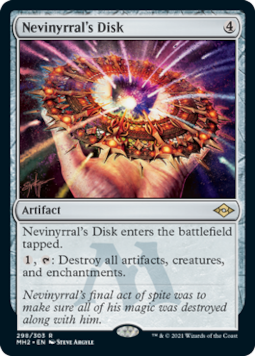
\includegraphics[width=0.25\textwidth]{assets/figure-magic-artifact}
 \end{figure}

 Fails when differences involve \emph{graphics and layout}.
\end{frame}

\begin{frame}[fragile]{Polymorphism / Visitor}
 Common \emph{wrong} or \emph{non optimal} approaches:
 
 \begin{center}
  \texttt{QWidget* Character::render()} member function
 \end{center}
 
 \begin{columns}
  \begin{column}{0.54\textwidth}
   \begin{lstlisting}[language=C++]
class Character {
 public:
  virtual QWidget* render() = 0;
};
\end{lstlisting}
  \end{column}
  \begin{column}{0.46\textwidth}
   \begin{lstlisting}[language=C++]
QWidget* Hero::render() {
  return new QLabel("Weapon Damage " + QString::number(weapon_damage));
};

QWidget* Monster::render(){
  return new QLabel("Weapon Damage " + QString::number(arms));
};
\end{lstlisting}
  \end{column}
 \end{columns}

 Introduces \emph{unwanted coupling} between model and GUI.
\end{frame}

\begin{frame}[fragile]{Polymorphism / Visitor}
 Common \emph{wrong} or \emph{non optimal} approaches:
 
 \begin{center}
  \texttt{QWidget* Character::render()} member function
 \end{center}
 
 Fails when:
 \begin{itemize}
  \item switching to a different framework (GTK, OpenGL...)
  \item showing different version of the same entity (thumbnail, teaser, fullscreen...)
  \item translating the GUI
 \end{itemize}
 
 ...and possibly more.
\end{frame}

\begin{frame}[fragile]{Polymorphism / Visitor}
 Common \emph{wrong} or \emph{non optimal} approaches:
 
 \begin{center}
  RTTI / dynamic cast / typeid
 \end{center}
 
 \begin{lstlisting}[language=C++]
Info::Info(Character& character, QWidget* parent) {
  ...
  Hero* hero = dynamic_cast<Hero*>(&character);
  if (hero != nullptr) { ... }
  
  Monster* monster = dynamic_cast<Monster*>(&character);
  if (monster != nullptr) { ... }
}
\end{lstlisting}
 
 Works for \emph{small hierarchies not changing over time}.
\end{frame}

\begin{frame}{Polymorphism / Visitor}
 Common \emph{wrong} or \emph{non optimal} approaches:
 
 \begin{center}
  RTTI / dynamic cast / typeid
 \end{center}
 
 Problems:
 \begin{itemize}
  \item when adding a subclass: \emph{remember} where RTTI was used
  \item \texttt{if} or \texttt{else if}?
  \item \emph{order} of checks matters
  \item \emph{multiple inheritance} can be complex
 \end{itemize}
 
 RTTI's slowness not an issue for GUIs.
\end{frame}

\begin{frame}[fragile]{Polymorphism / Visitor}
 Common \emph{wrong} or \emph{non optimal} approaches:
 
 \begin{center}
  \texttt{std::string Character::getType()} member function
 \end{center}
 
 \begin{lstlisting}[language=C++]
Info::Info(Character& character, QWidget* parent) {
  ...
  if (character.getType() == "hero") { ... }
  
  if (monster.getType() == "monster") { ... }
}
\end{lstlisting}
 
 A strictly \emph{worse version of RTTI}.
\end{frame}

\begin{frame}{Polymorphism / Visitor}
 Common \emph{wrong} or \emph{non optimal} approaches:
 
 \begin{center}
  \texttt{std::string Character::getType()} member function
 \end{center}
 
 Same problems as RTTI, plus:
 \begin{itemize}
  \item unchecked misspells
  \item hard-coded values
  \item must remember naming convention
  \item possible name clashes
 \end{itemize}
 
 \texttt{getType} is a way to fake polymorphism.
\end{frame}

\begin{frame}{Polymorphism / Visitor}
 Possible (correct) solution:
 
 \begin{center}
  Visitor
 \end{center}
 
 Core ideas:
 \begin{itemize}
  \item \emph{separate} data structure from visual representation
  \item dynamically \emph{extend} a class' capabilities
  \item compiler-assisted \emph{error checking}
  \item well-known \emph{design pattern}
 \end{itemize}
 
 ...at the cost of slightly \emph{more code}.
\end{frame}

\begin{frame}{Polymorphism / Visitor}
 Possible (correct) solution:
 
 \begin{center}
  Visitor
 \end{center}
 
 \begin{figure}
  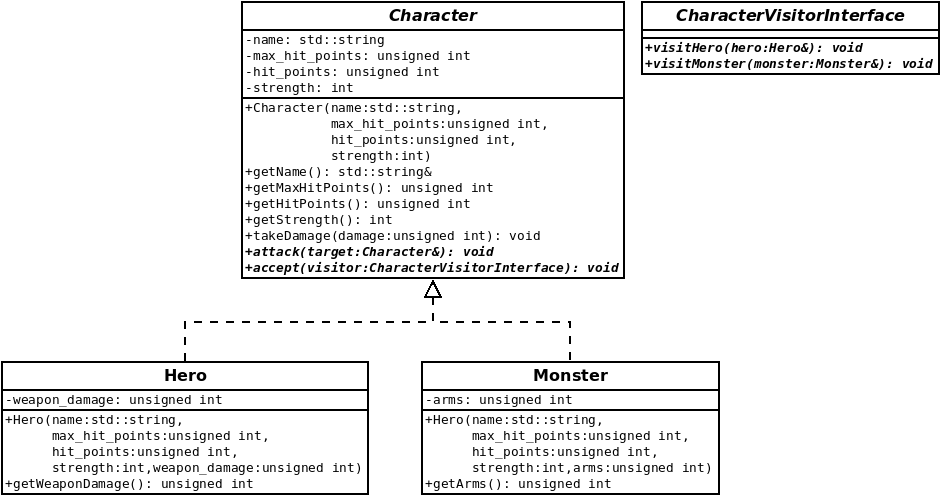
\includegraphics[width=0.75\textwidth]{assets/diagram-battle-scene-2}
 \end{figure}
 
 Visitors can perform actions depending on the concrete type.
\end{frame}

\begin{frame}[fragile]{Polymorphism / Visitor}
 Possible (correct) solution:
 
 \begin{center}
  Visitor
 \end{center}
 
  \begin{lstlisting}[language=C++]
void Hero::accept(CharacterVisitorInterface& visitor) {
  visitor.visitHero(*this);
}

void Monster::accept(CharacterVisitorInterface& visitor) {
  visitor.visitMonster(*this);
}
\end{lstlisting}
 
 Concrete classes choose right types.
\end{frame}

\begin{frame}[fragile]{Polymorphism / Visitor}
 Possible (correct) solution:
 
 \begin{center}
  Visitor
 \end{center}
 
  \begin{lstlisting}[language=C++]
class CharacterInfoVisitor: public Game::CharacterVisitorInterface {
 private:
  QWidget* widget;

 public:
  QWidget* getWidget();
  virtual void visitHero(Hero& hero);
  virtual void visitMonster(Monster& monster);
};
\end{lstlisting}
 
 A concrete visitor can build a suitable widget.
\end{frame}

\begin{frame}[fragile]{Polymorphism / Visitor}
 Possible (correct) solution:
 
 \begin{center}
  Visitor
 \end{center}
 
  \begin{lstlisting}[language=C++]
QWidget* CharacterInfoVisitor::getWidget() {
  return widget;
}

void CharacterInfoVisitor::visitHero(Hero& hero) {
  widget = new QLabel("Weapon Damage: " + QString::number(hero.getWeaponDamage()));
}

void CharacterInfoVisitor::visitMonster(Monster& monster) {
  widget = new QLabel("Arms Multiplier: " + QString::number(monster.getArms()));
}
\end{lstlisting}
 
 A concrete visitor can build a suitable widget.
\end{frame}

\begin{frame}[fragile]{Polymorphism / Visitor}
 Possible (correct) solution:
 
 \begin{center}
  Visitor
 \end{center}
 
  \begin{lstlisting}[language=C++]
Info::Info(Character& character, QWidget* parent)
  : QWidget(parent), character(character)
{
  ...
  strength_label = new QLabel();
  layout->addWidget(strength_label);
  
  CharacterInfoVisitor visitor;
  character.accept(visitor);
  layout->addWidget(visitor.getWidget());
}
\end{lstlisting}
 
 The caller must use the Visitor.
\end{frame}

\begin{frame}[fragile]{Polymorphism / Visitor}
 Possible (correct) solution:
 
 \begin{center}
  Visitor
 \end{center}
 
 Advantages:
 \begin{itemize}
  \item \emph{error-checking} through subclassing
  \item complete \emph{separation} between model and GUI
  \item Visitors can be used for \emph{different purposes}
  \item different Visitors for \emph{different layouts/frameworks}
  \item Visitors can have \emph{internal state}
 \end{itemize}
 
 Disadvantage: more \emph{boilerplate code}.
\end{frame}

\begin{frame}{Polymorphism / Visitor}
 A visitor is a \emph{formal but complex} solution: use what suits the context best!
 
 \begin{columns}
  \begin{column}{0.15\textwidth}
   \includegraphics[width=0.99\textwidth]{assets/logo-github}
  \end{column}
  \begin{column}{0.85\textwidth}
   Source code available at:
   \url{https://github.com/Unipd-Object-Oriented-Programming/game/tree/visitor}
  \end{column}
 \end{columns}
 
 More about Visitors: \href{https://en.wikipedia.org/wiki/Visitor_pattern}{Wikipedia/Visitor pattern}.
\end{frame}

\begin{frame}[fragile]{Polymorphism / Observer}
 \texttt{Info} must be updated when character takes damage:
 
 \begin{lstlisting}[language=C++]
void Battle::playerAttacks() {
  hero.attack(monster);
  monster_panel->refresh();
  // will call info->show();
  
  monster.attack(hero);
  hero_panel->refresh();
  // will call info->show();
}
\end{lstlisting}
 
 Recurring problem: update view upon \emph{content changes}.
\end{frame}

\begin{frame}{Polymorphism / Observer}
 The problem:
 
 \begin{itemize}
  \item \texttt{Info} \emph{should be bound} to a \texttt{Character}
  \item \texttt{Info} \emph{should automatically update} when \texttt{Character} changes
  \item current approach bloats \texttt{Battle} with \emph{view update logic}
 \end{itemize}
 
 Solution:
 \begin{itemize}
  \item \emph{remove view update} logic from \texttt{Battle}
  \item \emph{bind} \texttt{Info} to its \texttt{Character}
  \item let \texttt{Character} \emph{notify} its \texttt{Info} upon state changes
 \end{itemize}
 
 \texttt{Info} is \emph{observing} \texttt{Character}.
\end{frame}

\begin{frame}{Polymorphism / Observer}
 The \emph{Observer} pattern:
 \begin{figure}
  \includegraphics[width=0.75\textwidth]{assets/diagram-battle-scene-3}
 \end{figure}
 
 Observers \emph{register} to characters, which \emph{notify} them.
\end{frame}

\begin{frame}[fragile]{Polymorphism / Observer}
 The \emph{Observer} pattern:

 \begin{lstlisting}[language=C++]
class CharacterObserverInterface {
 public:
  virtual ~CharacterObserverInterface() = default;
  virtual void notify(Character& character) = 0;
};
\end{lstlisting}

 \texttt{Observer} receive updated \texttt{Character} and takes action.
\end{frame}

\begin{frame}[fragile]{Polymorphism / Observer}
 The \emph{Observer} pattern:

 \begin{lstlisting}[language=C++]
class Character {
 private:
  ...
  std::vector<CharacterObserverInterface*> observers;

 public:
  ...
  void registerObserver(CharacterObserverInterface* obs);
};
\end{lstlisting}

 \texttt{Observer}s register to a \texttt{Character}, which stores them.
\end{frame}

\begin{frame}[fragile]{Polymorphism / Observer}
 The \emph{Observer} pattern:

 \begin{lstlisting}[language=C++]
void Character::takeDamage(const unsigned int damage) {
  hit_points = (damage > hit_points) ? 0 : hit_points - damage;
  for (auto observer = observers.begin(); observer != observers.end(); observer++) {
      (*observer)->notify(*this);
  }
}

void Character::registerObserver(CharacterObserverInterface* observer) {
  observers.push_back(observer);
}
\end{lstlisting}

 \texttt{Character} knows when to \texttt{notify} \texttt{Observer}s.
\end{frame}

\begin{frame}[fragile]{Polymorphism / Observer}
 The \emph{Observer} pattern:

 \begin{lstlisting}[language=C++]
class Info: public QWidget, public CharacterObserverInterface {
  ...

 public:
  Info(Character& character, QWidget* parent = 0);
  void show();
  virtual void notify(Character& character);
};
\end{lstlisting}

 \texttt{Info} is now an \texttt{Observer}.
\end{frame}


\begin{frame}[fragile]{Polymorphism / Observer}
 The \emph{Observer} pattern:

 \begin{lstlisting}[language=C++]
Info::Info(Character& character, QWidget* parent)
    : QWidget(parent), character(character)
{
  QVBoxLayout* layout = new QVBoxLayout(this);
  layout->setAlignment(Qt::AlignLeft | Qt::AlignTop);
  ...
  character.registerObserver(this);
}

void Info::notify(Character& character) {
  hit_points_label->setText("HP: " + QString::number(character.getHitPoints()) + "/" + QString::number(character.getMaxHitPoints()));
}
\end{lstlisting}

 \texttt{Info} is now an \texttt{Observer}.
\end{frame}


\begin{frame}[fragile]{Polymorphism / Observer}
 The \emph{Observer} pattern:

 \begin{lstlisting}[language=C++]
class HeroPanel: public QWidget {
  Q_OBJECT
 private:
  QLabel* artwork;
  Info* info;
  
 public:
  HeroPanel(Game::Hero& hero, QWidget* parent = 0);
  
 signals:
  void attack();
};
\end{lstlisting}

\texttt{HeroPanel::refresh} and \texttt{MonsterPanel::refresh} no longer needed.
\end{frame}


\begin{frame}[fragile]{Polymorphism / Observer}
 The \emph{Observer} pattern:

 \begin{lstlisting}[language=C++]
void Battle::playerAttacks() {
  hero.attack(monster);
  monster.attack(hero);
}
\end{lstlisting}

\texttt{HeroPanel::refresh} and \texttt{MonsterPanel::refresh} no longer needed.
\end{frame}

\begin{frame}{Polymorphism / Observer}
 An observer is a \emph{formal but complex} solution: use what suits the context best!
 
 \begin{columns}
  \begin{column}{0.15\textwidth}
   \includegraphics[width=0.99\textwidth]{assets/logo-github}
  \end{column}
  \begin{column}{0.85\textwidth}
   Source code available at:
   \url{https://github.com/Unipd-Object-Oriented-Programming/game/tree/observer}
  \end{column}
 \end{columns}
 
 More about Visitors: \href{https://en.wikipedia.org/wiki/Observer_pattern}{Wikipedia/Observer pattern}.
\end{frame}

\end{document}
